\chapter{Le trek du Salkantay vers le Machu Picchu}
\section*{2 juin 2015}
Le trek du Salkantay en 6 jours (4 jours de trek, 1 jour pour visiter le Machu Picchu et 1 jour pour rentrer) : 174 dollars tout inclus avec l´option pour monter en haut de la montagne du Machu Picchu. \newline
 Jour 1 : \newline
 Trajet Cusco-Mollepata en bus puis en camion jusqu'au départ du trek. \newline
 \newline
\centerline{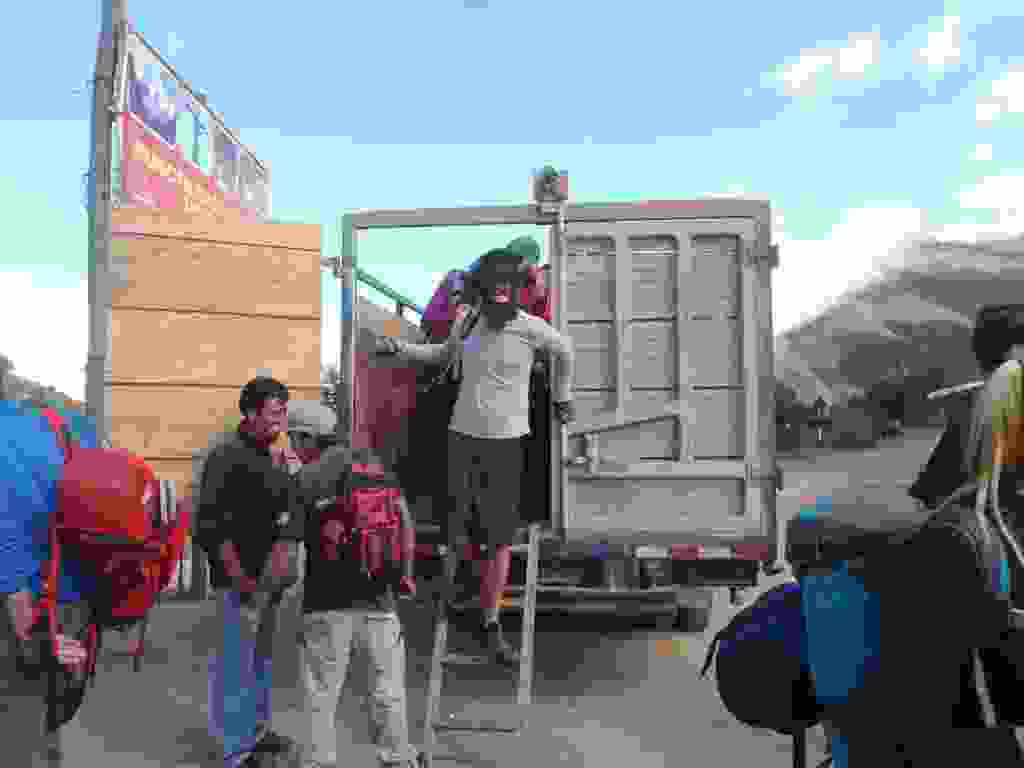
\includegraphics[width=\mywidth]{../wp-content/uploads/2015/05/P5234337-1024x768.jpg} } 
 \newline
 Belle montée pour atteindre le premier campement à 3900m. \newline
 \newline
\centerline{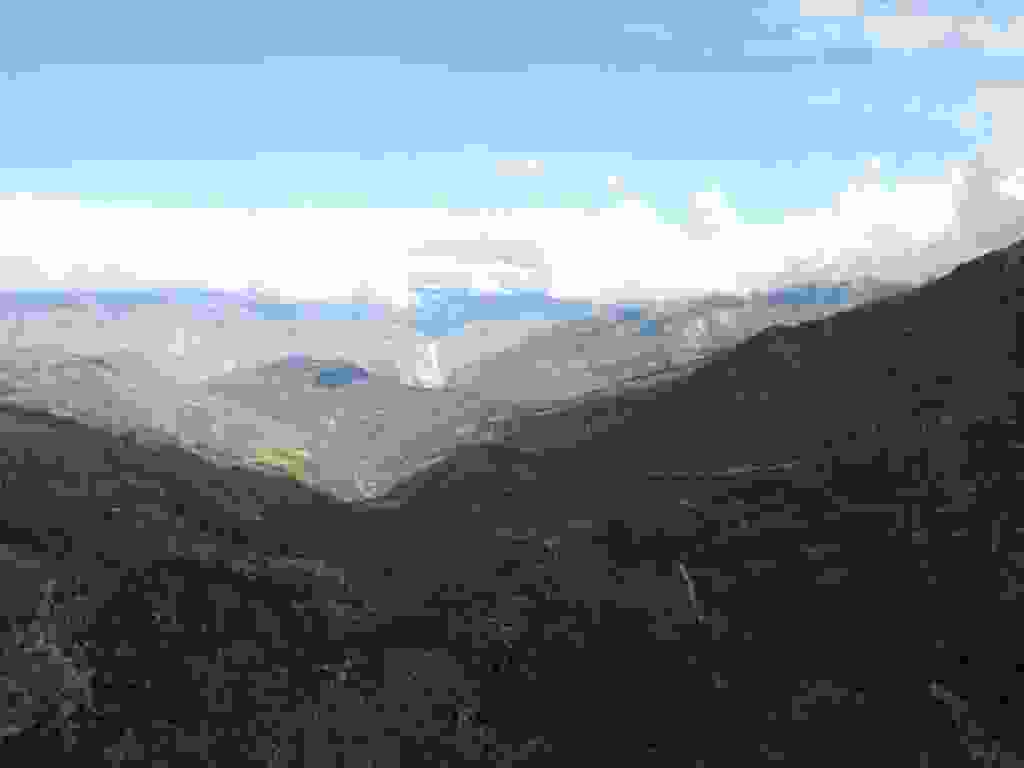
\includegraphics[width=\mywidth]{../wp-content/uploads/2015/05/P5234342-1024x768.jpg} } 
 \newline
 \newline
\centerline{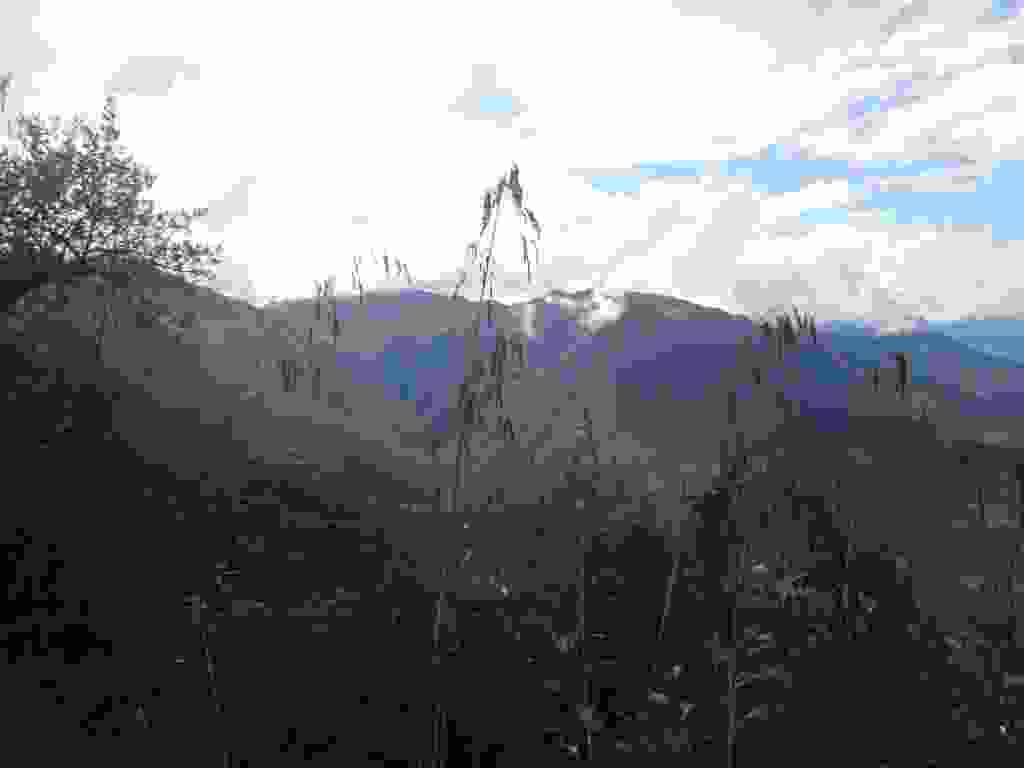
\includegraphics[width=\mywidth]{../wp-content/uploads/2015/05/P5234343-1024x768.jpg} } 
 \newline
 \newline
\centerline{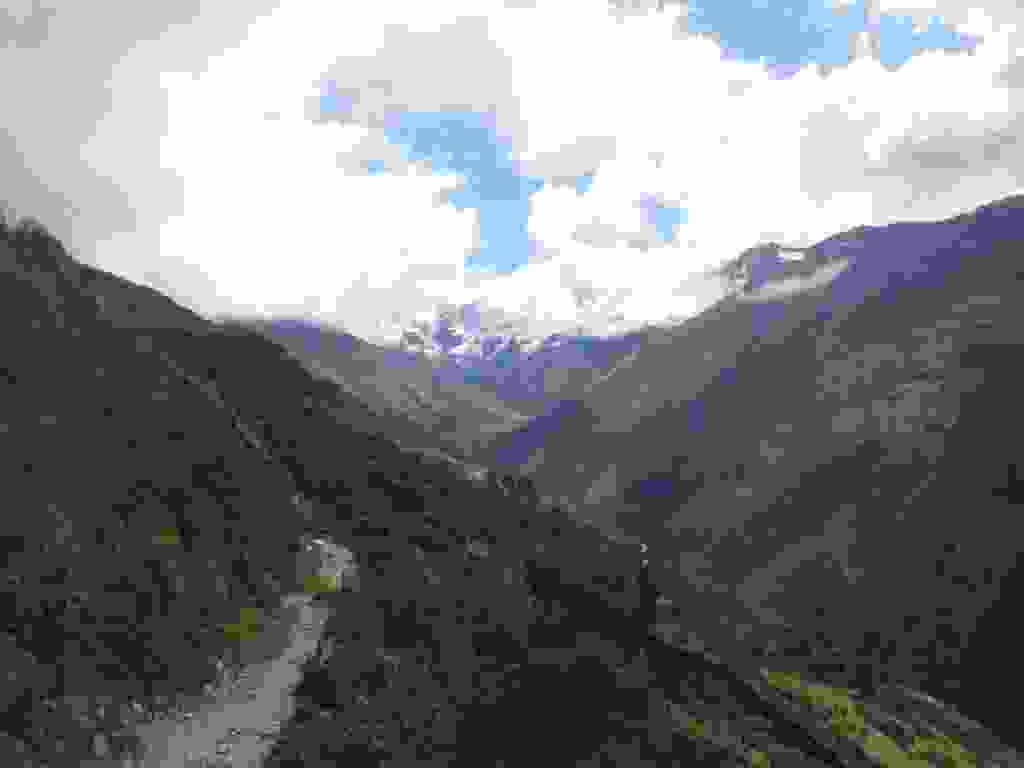
\includegraphics[width=\mywidth]{../wp-content/uploads/2015/05/P5234346-1024x768.jpg} } 
 \newline
 On commence a voir le glacier du Salkantay. \newline
 \newline
\centerline{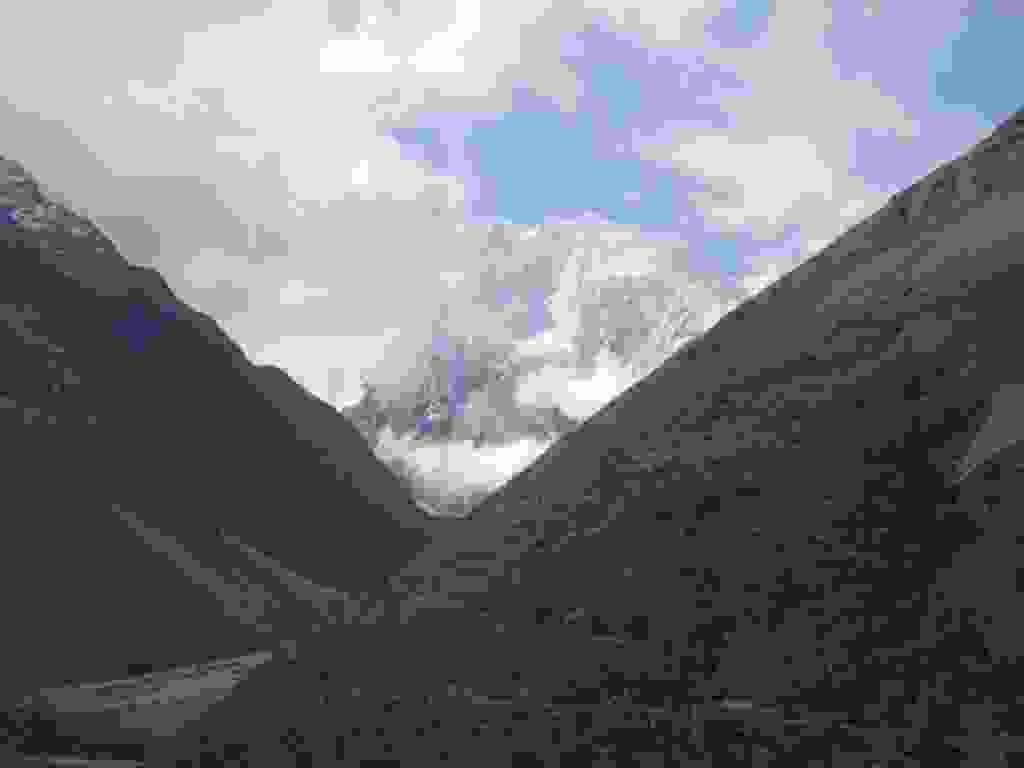
\includegraphics[width=\mywidth]{../wp-content/uploads/2015/05/P5234353-1024x768.jpg} } 
 \newline
 L'après midi aller retour pour voir un lac au pied du glacier Umantay. \newline
 \newline
\centerline{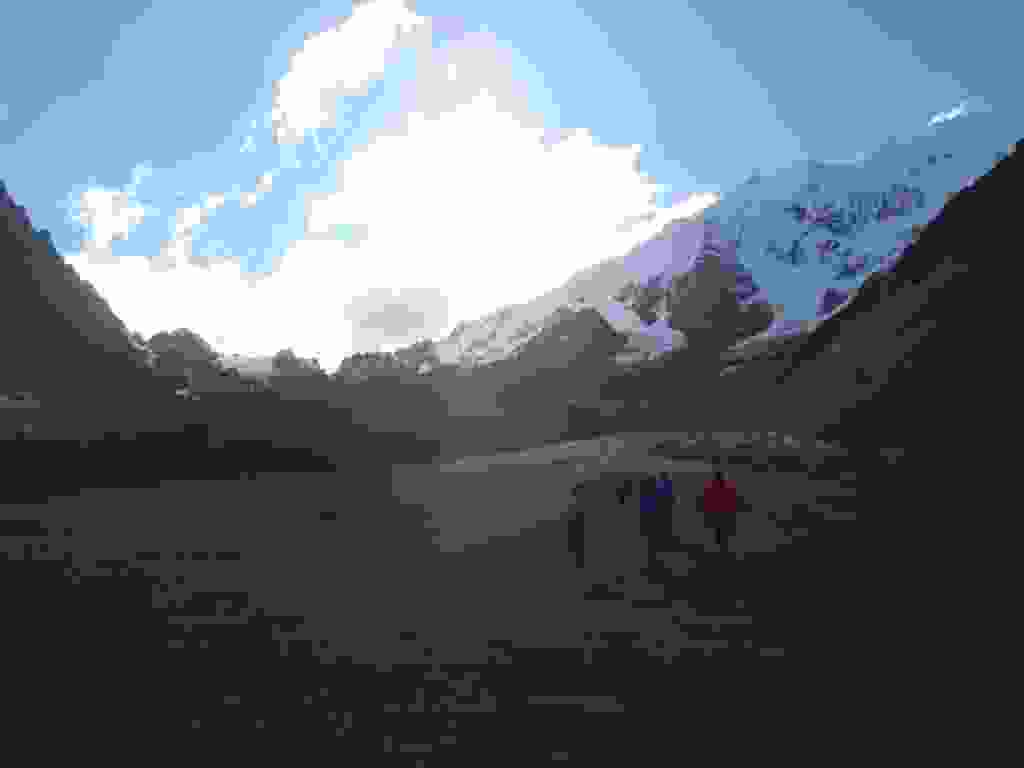
\includegraphics[width=\mywidth]{../wp-content/uploads/2015/05/P5234357-1024x768.jpg} } 
 \newline
 \newline
\centerline{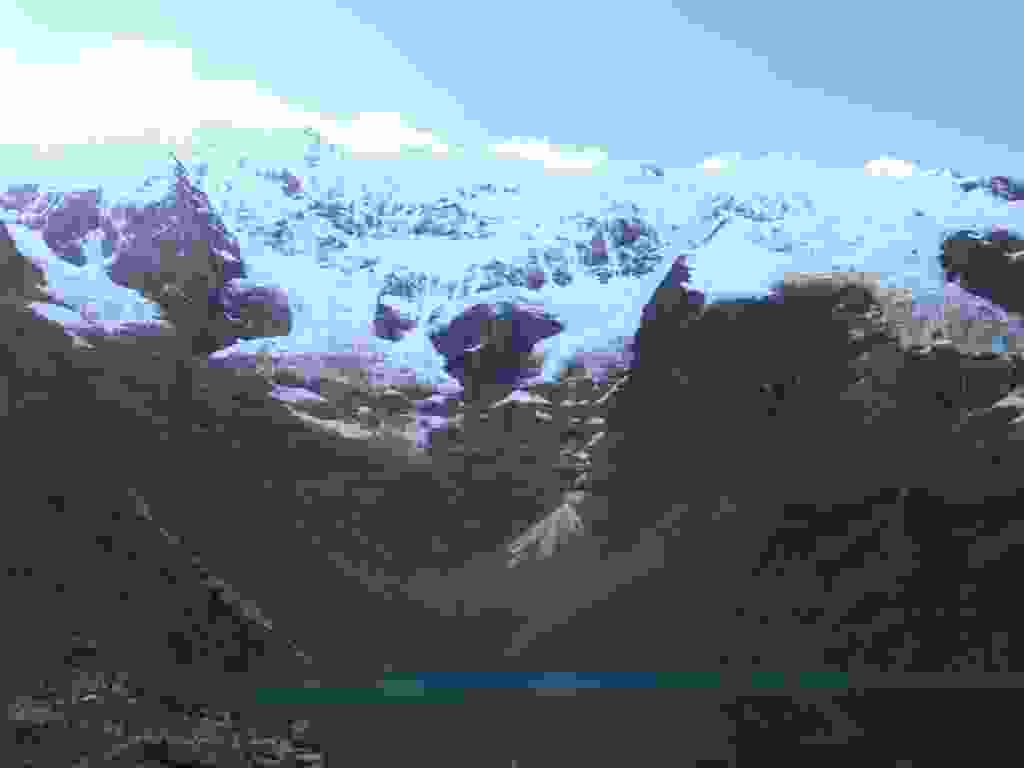
\includegraphics[width=\mywidth]{../wp-content/uploads/2015/05/P5234362-1024x768.jpg} } 
 \newline
 \newline
\centerline{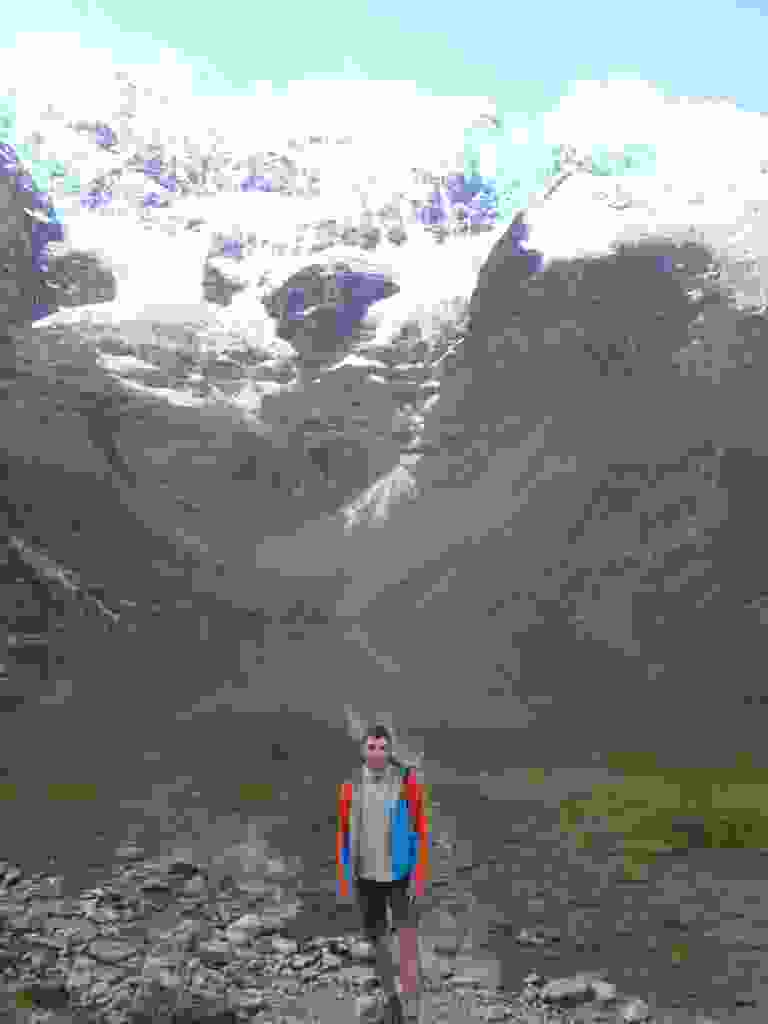
\includegraphics[width=\mywidth]{../wp-content/uploads/2015/05/P5234366-768x1024.jpg} } 
 \newline
 Jour 2 : \newline
 Lever à 5h et grosse montée. \newline
 \newline
\centerline{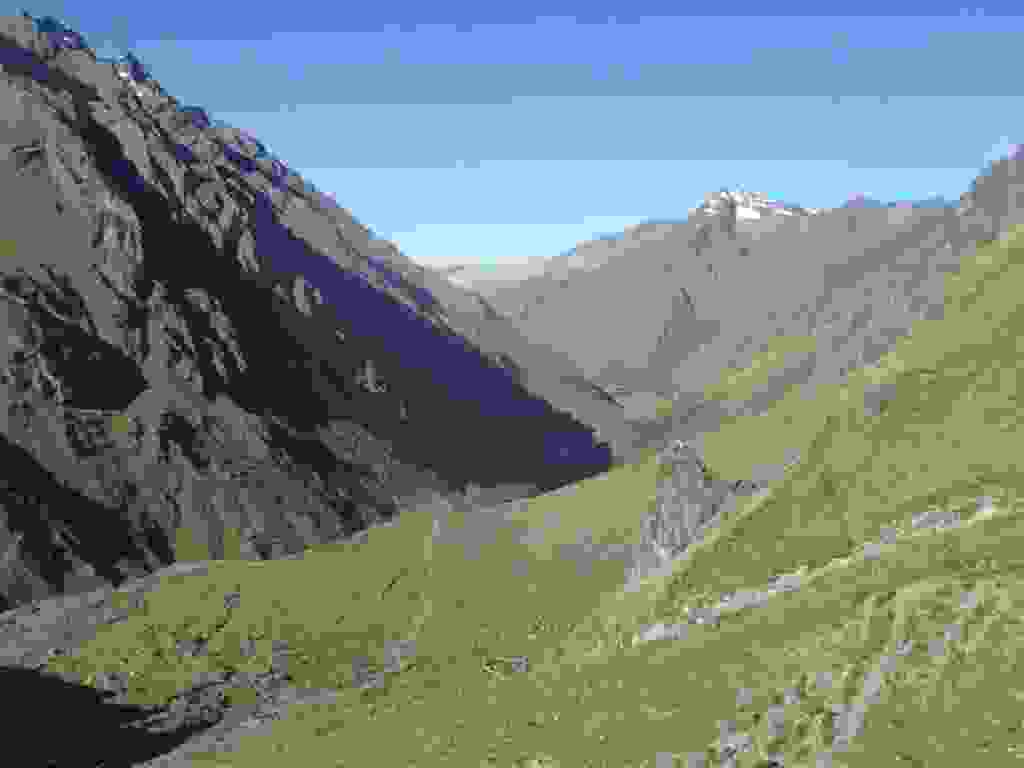
\includegraphics[width=\mywidth]{../wp-content/uploads/2015/05/P5244381-1024x768.jpg} } 
 \newline
 Le col du Salkantay à 4600m \newline
 \newline
\centerline{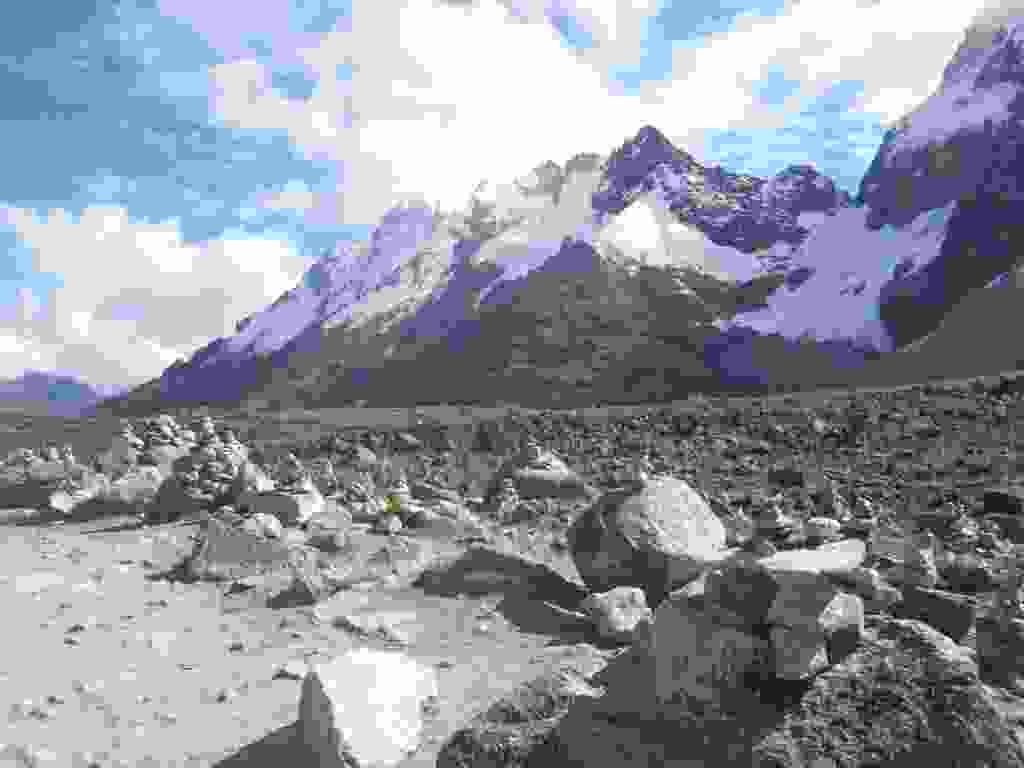
\includegraphics[width=\mywidth]{../wp-content/uploads/2015/05/P5244391-1024x768.jpg} } 
 \newline
 \newline
\centerline{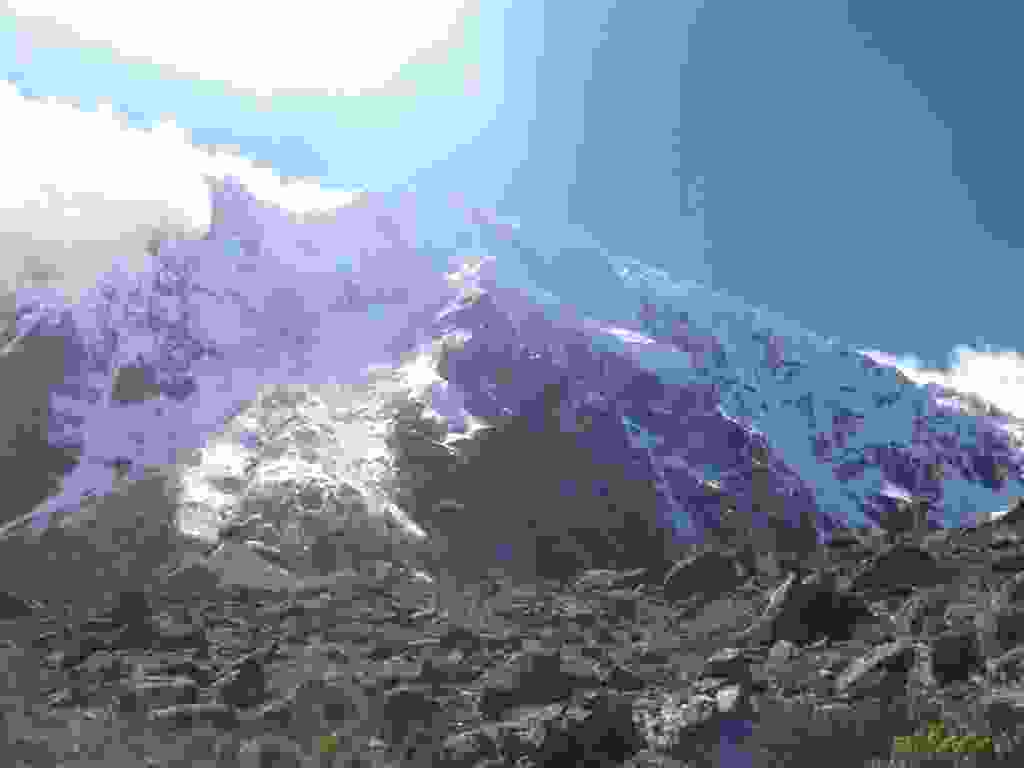
\includegraphics[width=\mywidth]{../wp-content/uploads/2015/05/P5244400-1024x768.jpg} } 
 \newline
 Le groupe au sommet avec notre guide Jean Paul. \newline
 \newline
\centerline{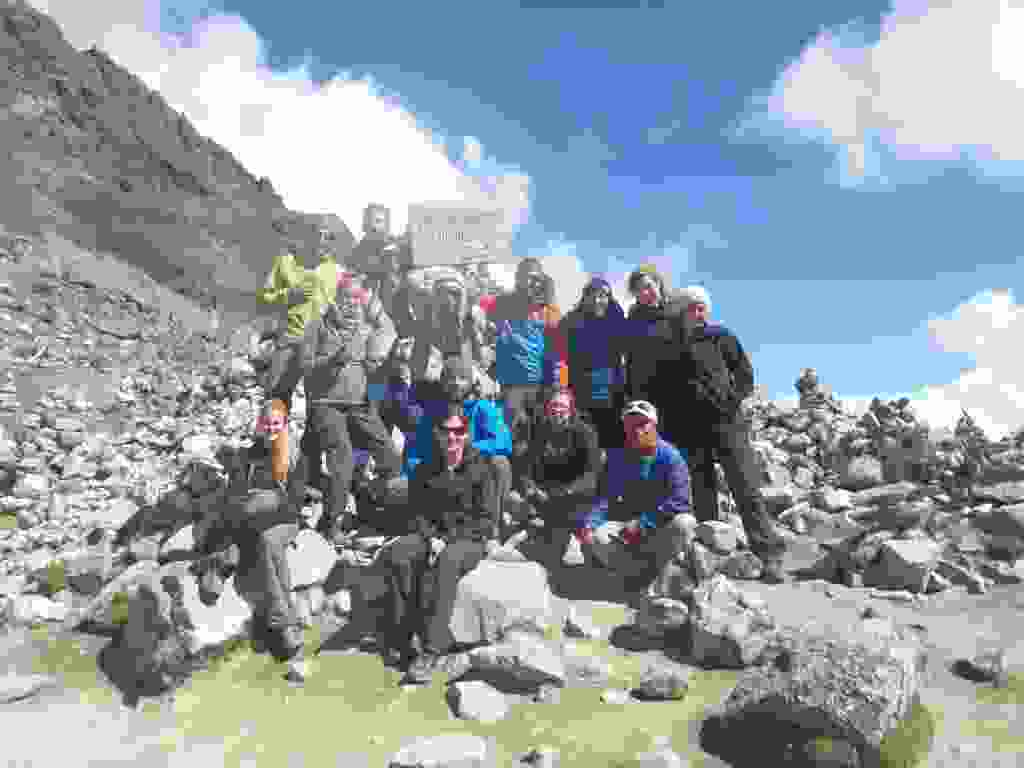
\includegraphics[width=\mywidth]{../wp-content/uploads/2015/05/P5244396-1024x768.jpg} } 
 \newline
 La nourriture et les tentes sont portées par des chevaux. \newline
 \newline
\centerline{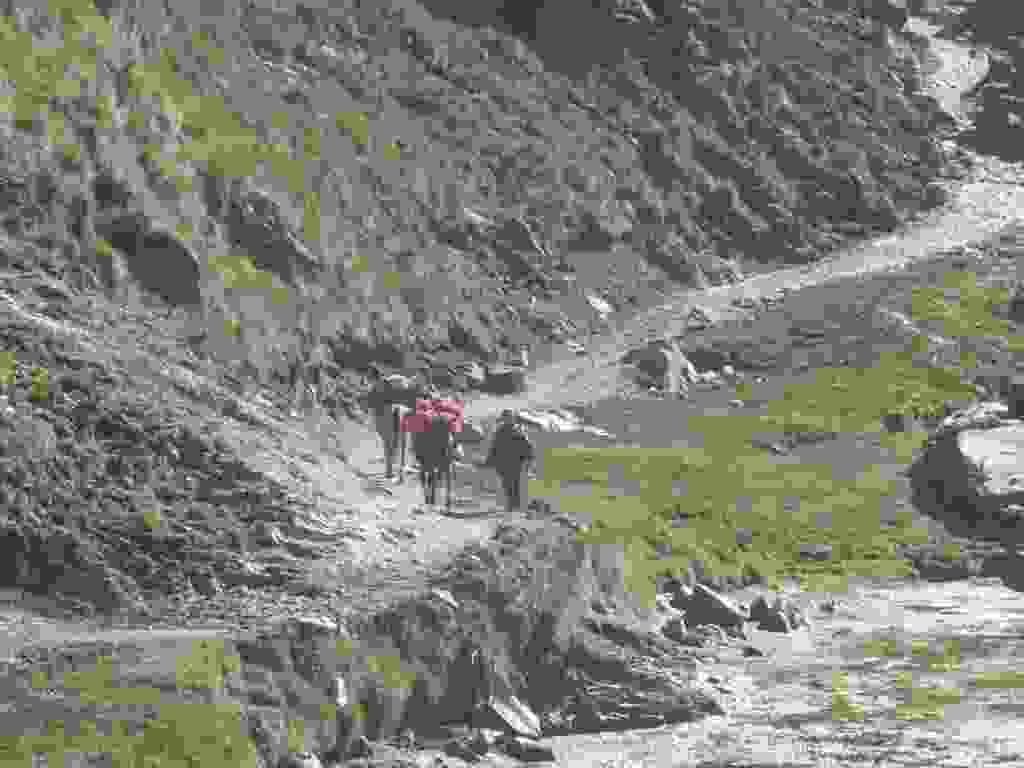
\includegraphics[width=\mywidth]{../wp-content/uploads/2015/05/P5244386-1024x768.jpg} } 
 \newline
 Longue descente jusqu´au 2e camp a 2900m. Petit a petit on se rapproche de la jungle. \newline
 \newline
\centerline{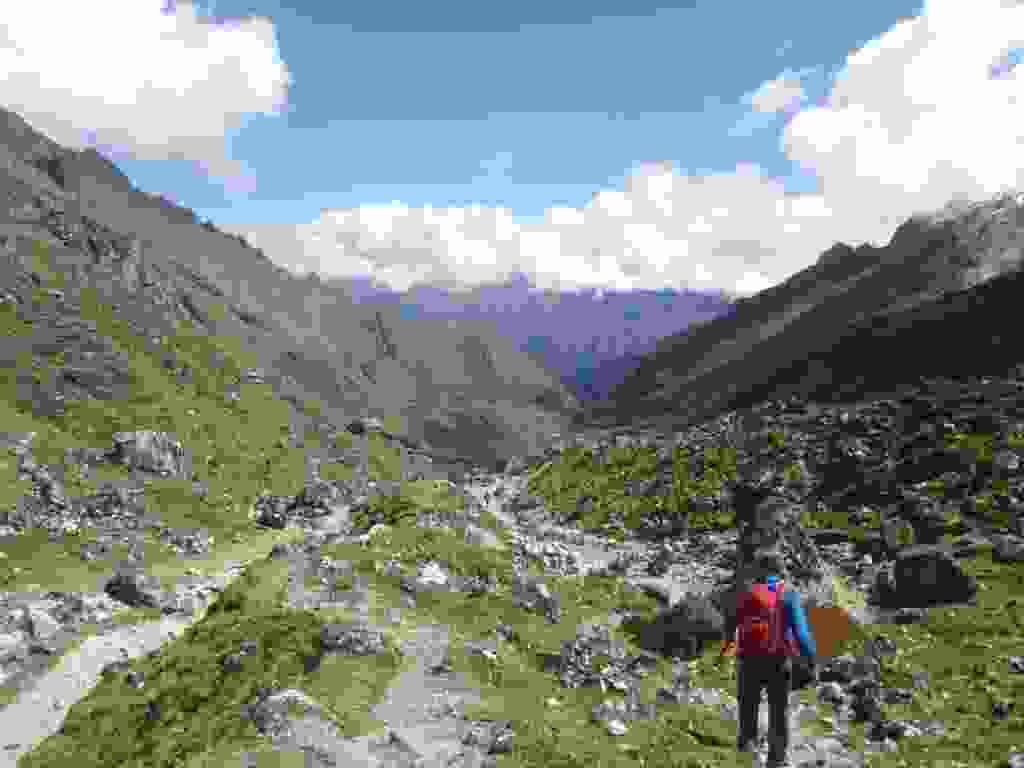
\includegraphics[width=\mywidth]{../wp-content/uploads/2015/05/P5244403-1024x768.jpg} } 
 \newline
 \newline
\centerline{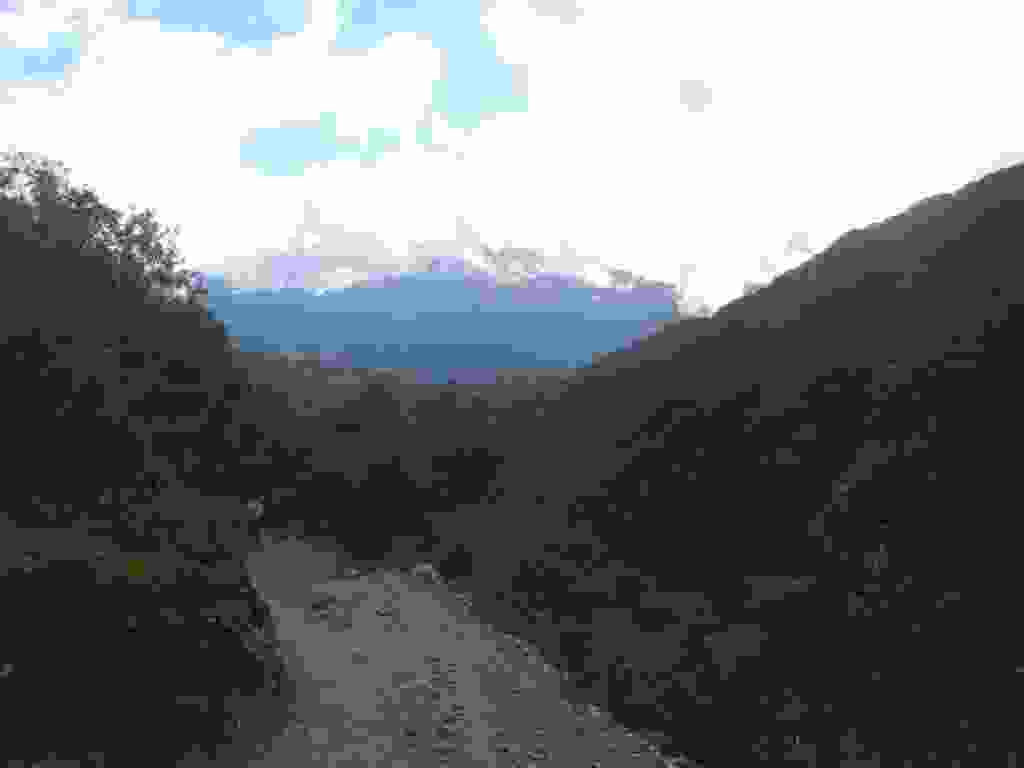
\includegraphics[width=\mywidth]{../wp-content/uploads/2015/05/P5244409-1024x768.jpg} } 
 \newline
 \newline
\centerline{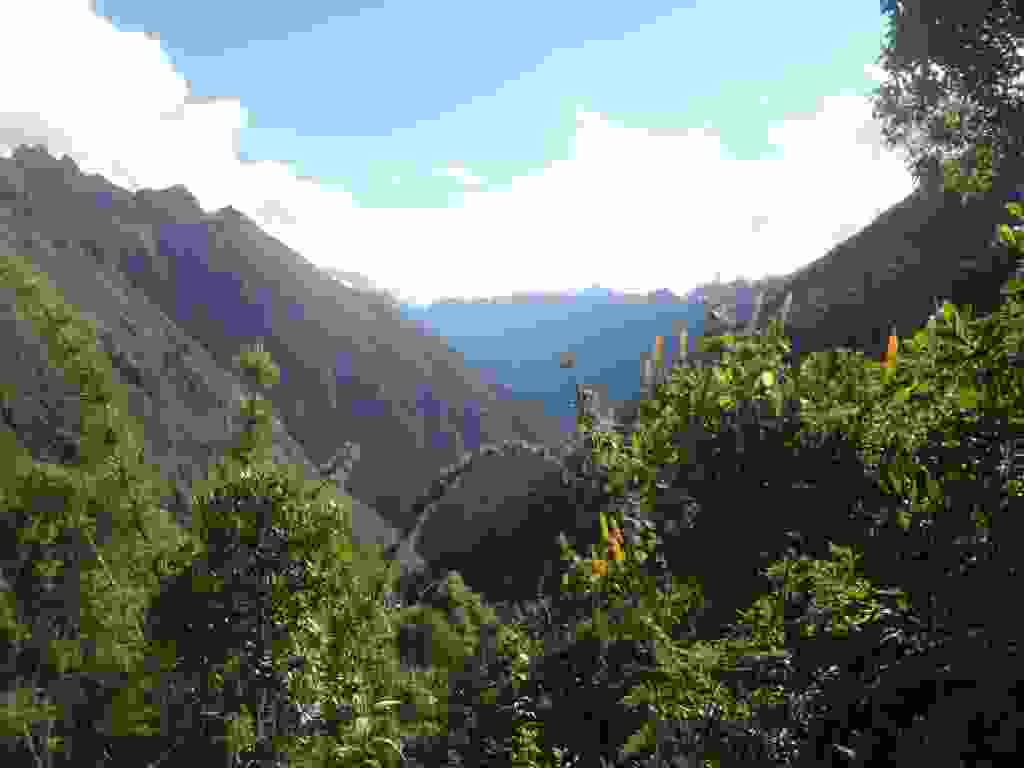
\includegraphics[width=\mywidth]{../wp-content/uploads/2015/05/P5244414-1024x768.jpg} } 
 \newline
 \newline
\centerline{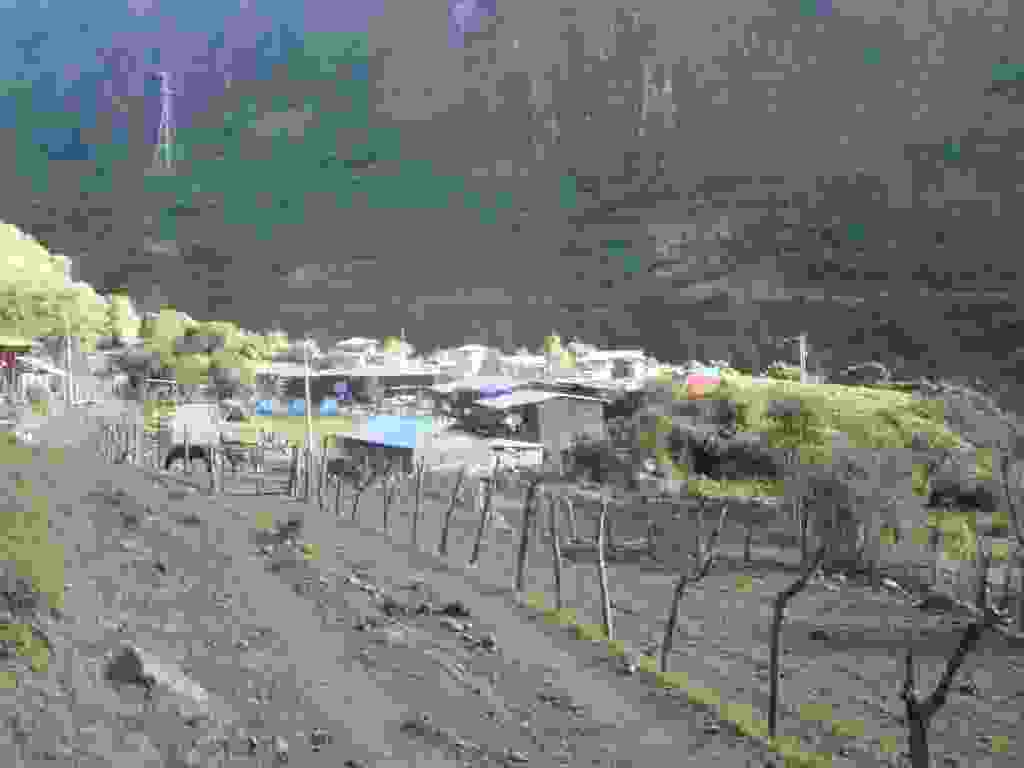
\includegraphics[width=\mywidth]{../wp-content/uploads/2015/05/P5244415-1024x768.jpg} } 
 \newline
 Jour 3 : \newline
 Notre groupe s´appelait «Les Condors» pour le trek. \newline
 \newline
\centerline{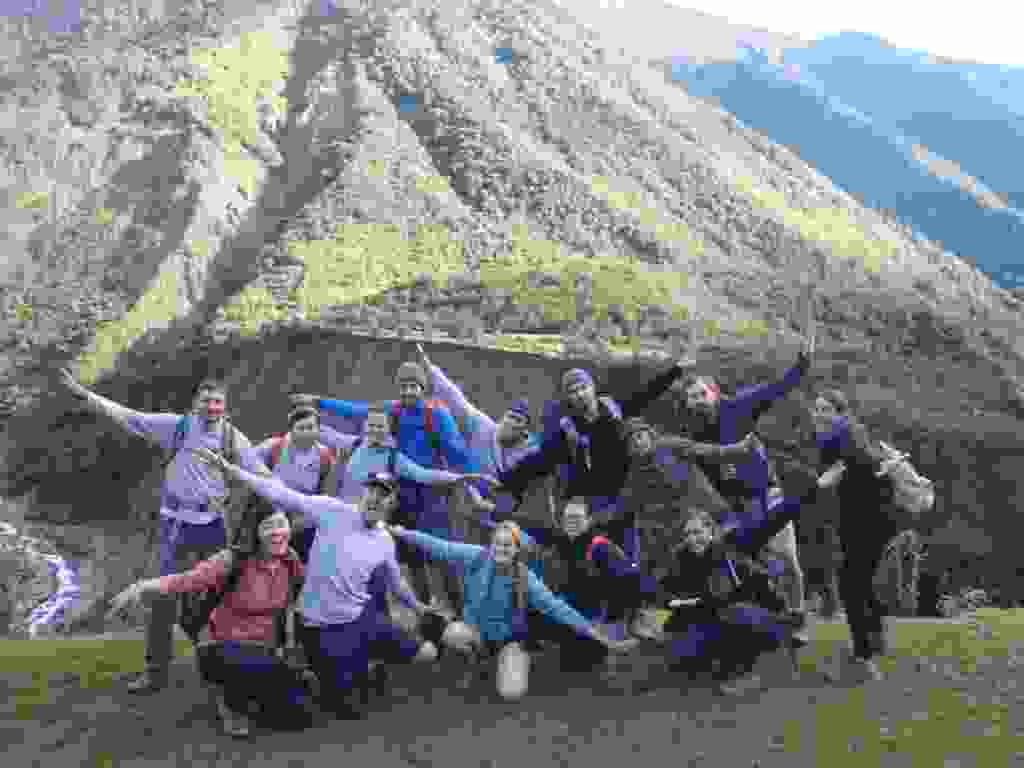
\includegraphics[width=\mywidth]{../wp-content/uploads/2015/05/P5254421-1024x768.jpg} } 
 \newline
 On était un peu de tous les pays : France, Allemagne, Angleterre, Canada, Israël, République tchèque, ca fait parler anglais. \newline
 Le chemin alterne montées et descentes au milieu d'une végétation très dense. \newline
 \newline
\centerline{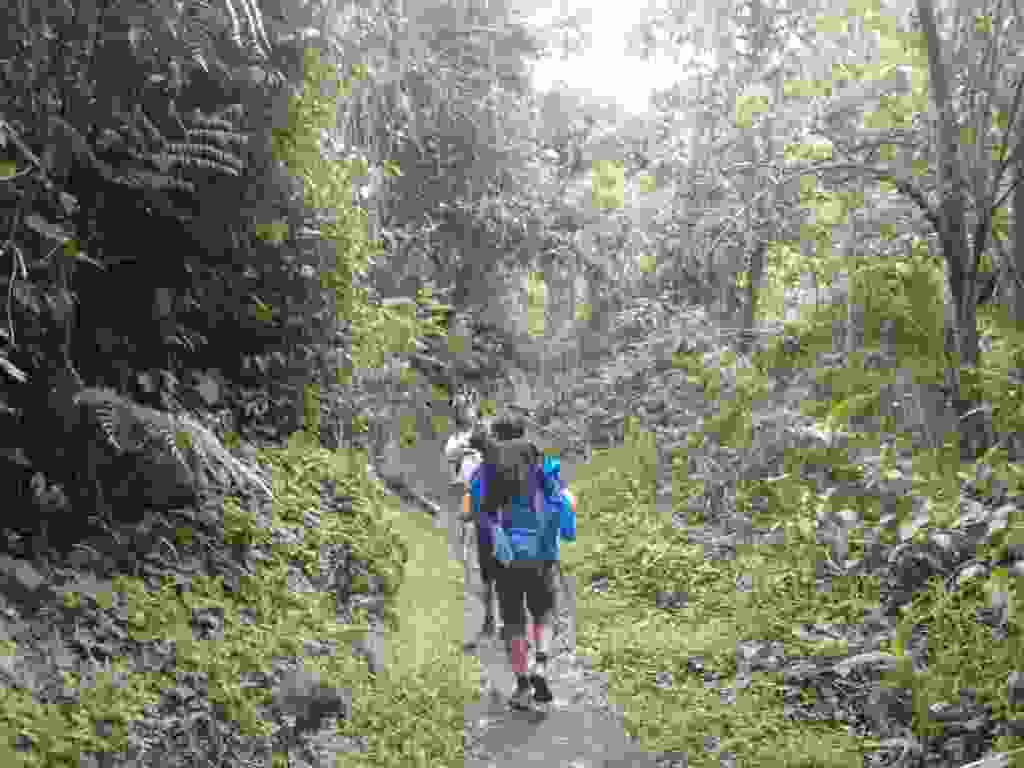
\includegraphics[width=\mywidth]{../wp-content/uploads/2015/05/P5254428-1024x768.jpg} } 
 \newline
 \newline
\centerline{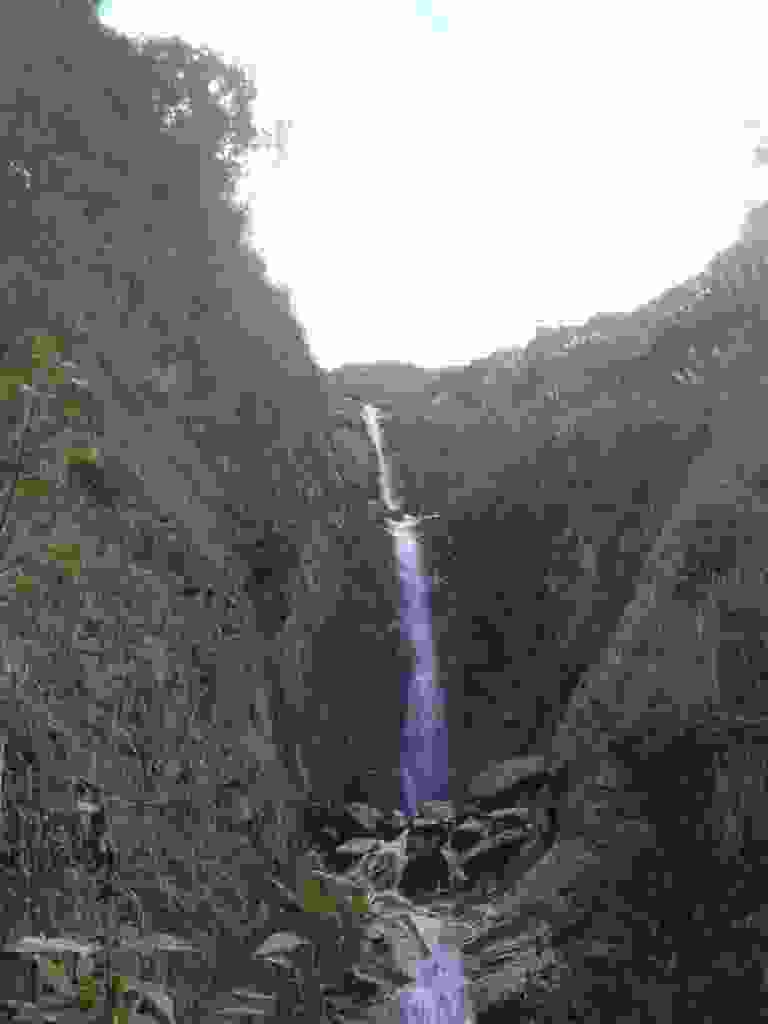
\includegraphics[width=\mywidth]{../wp-content/uploads/2015/05/P5254424-768x1024.jpg} } 
 \newline
 On croise quelques arbres fruitiers. \newline
 \newline
\centerline{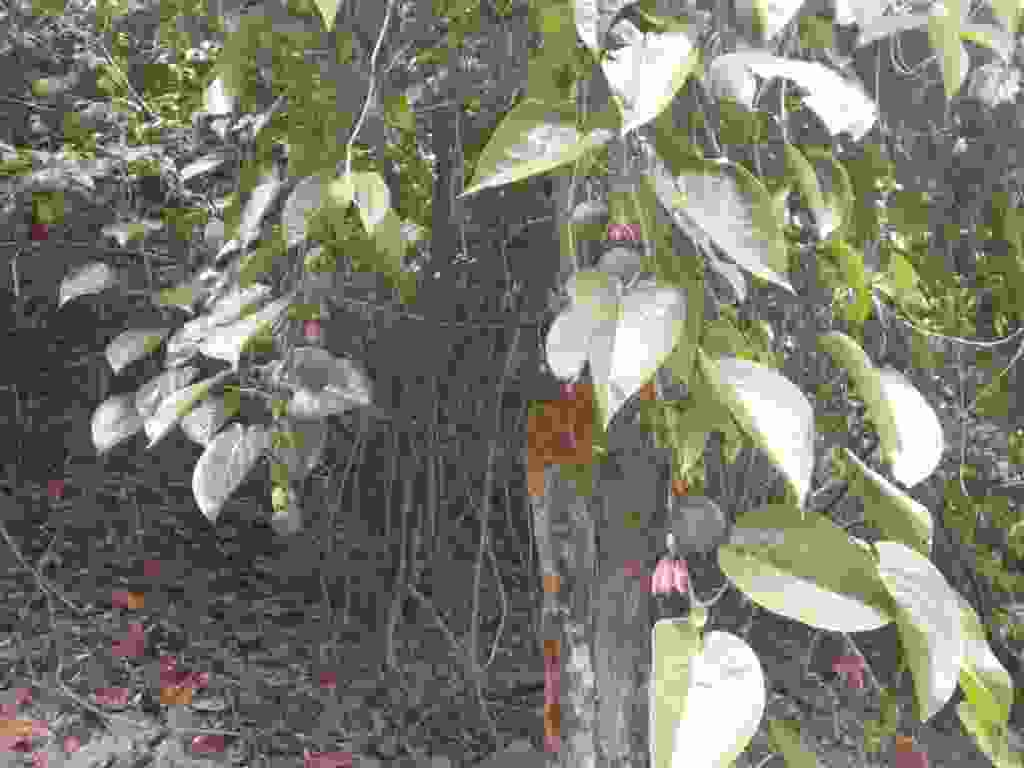
\includegraphics[width=\mywidth]{../wp-content/uploads/2015/05/P5254427-1024x768.jpg} } 
 \newline
 \newline
\centerline{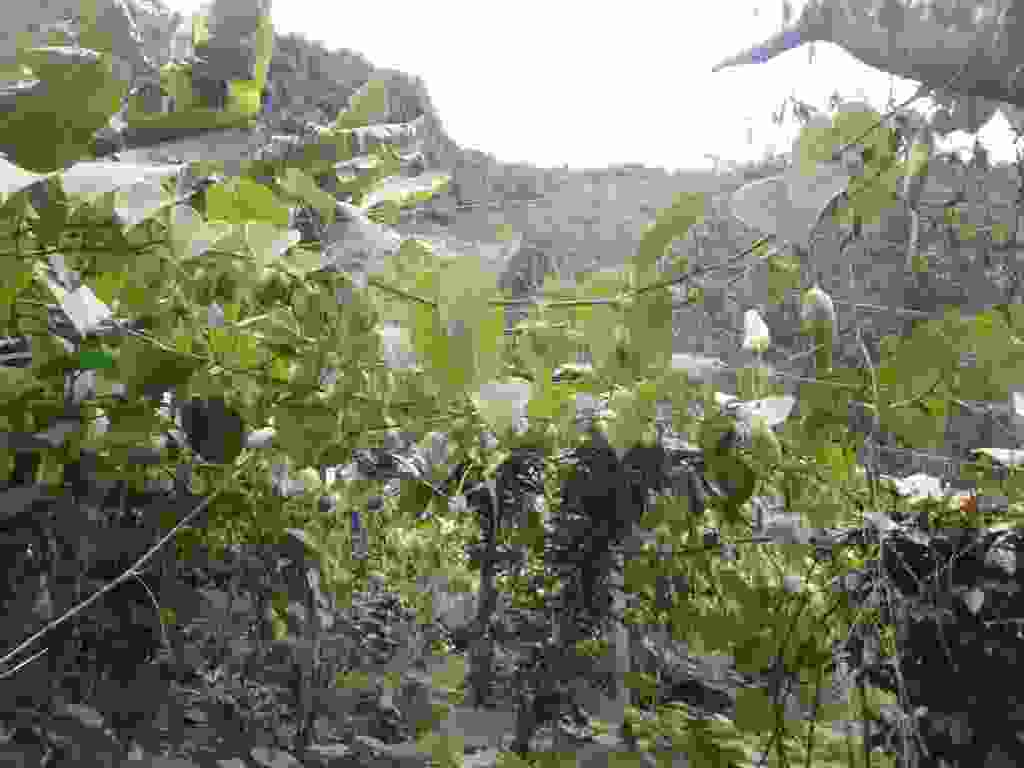
\includegraphics[width=\mywidth]{../wp-content/uploads/2015/05/P5254430-1024x768.jpg} } 
 \newline
 \newline
\centerline{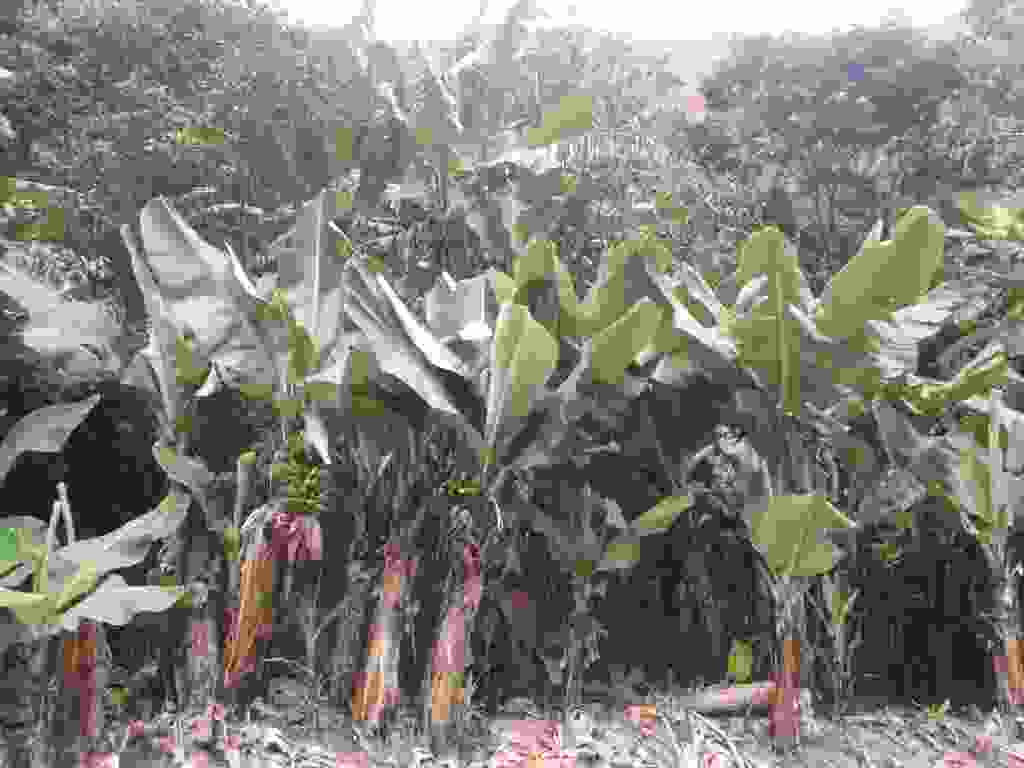
\includegraphics[width=\mywidth]{../wp-content/uploads/2015/05/P5264440-1024x768.jpg} } 
 \newline
 Repas de midi à Santa Maria : le cuisiner du trek nous gâte avec des spécialités péruviennes, ceviche et papas rellenas. \newline
 \newline
\centerline{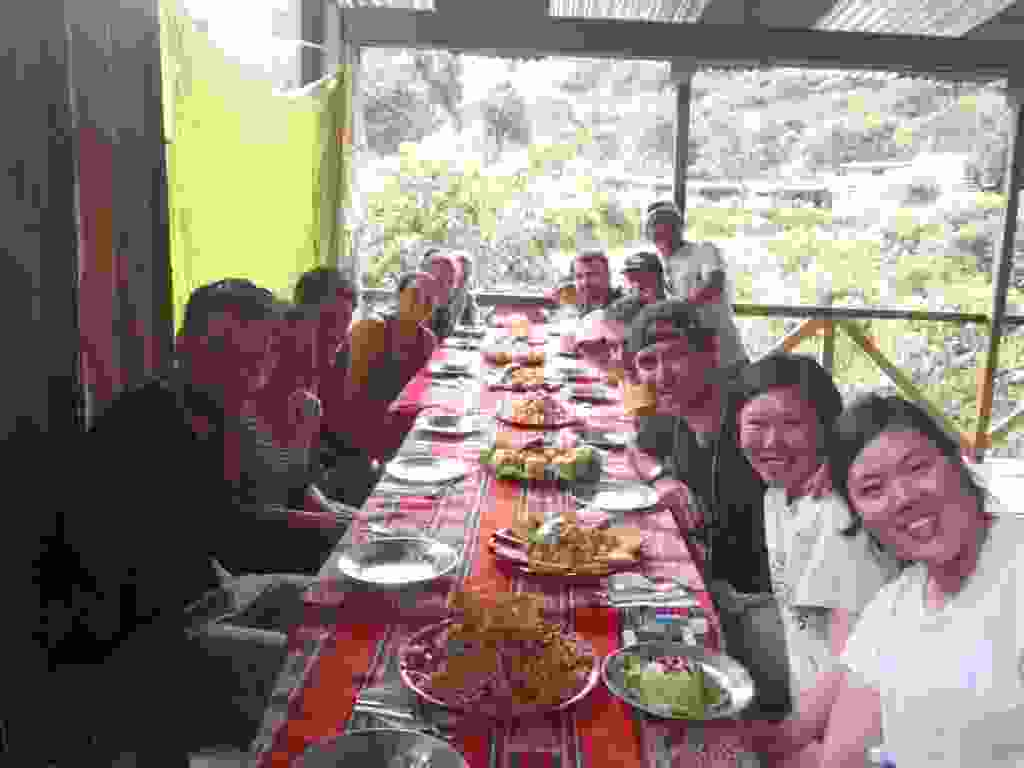
\includegraphics[width=\mywidth]{../wp-content/uploads/2015/05/P5254431-1024x768.jpg} } 
 \newline
 Un bon moment aux bains de Santa Teresa. \newline
 \newline
\centerline{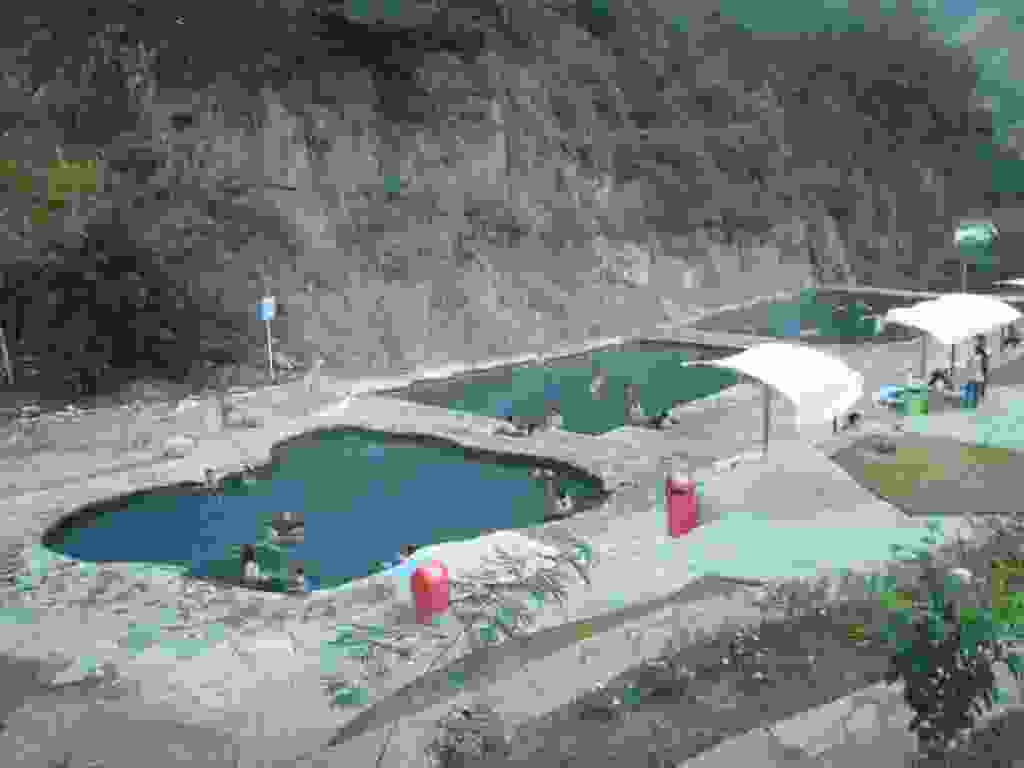
\includegraphics[width=\mywidth]{../wp-content/uploads/2015/05/P5264435-1024x768.jpg} } 
 \newline
 Jour 4 : \newline
 Le matin marche sur la route pour arriver à Hidroelectrica. \newline
 \newline
\centerline{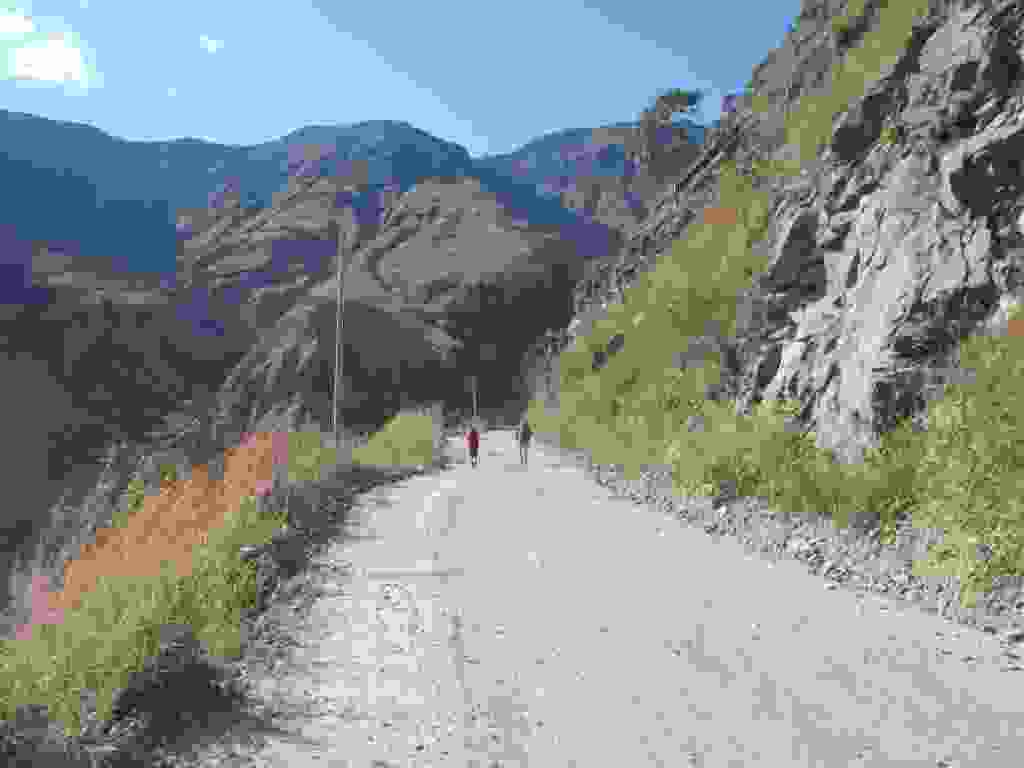
\includegraphics[width=\mywidth]{../wp-content/uploads/2015/05/P5264437-1024x768.jpg} } 
 \newline
 L'après midi, le long de la voie ferrée jusqu'au village en bas du Machu Picchu : Aguas Calientes. \newline
 \newline
\centerline{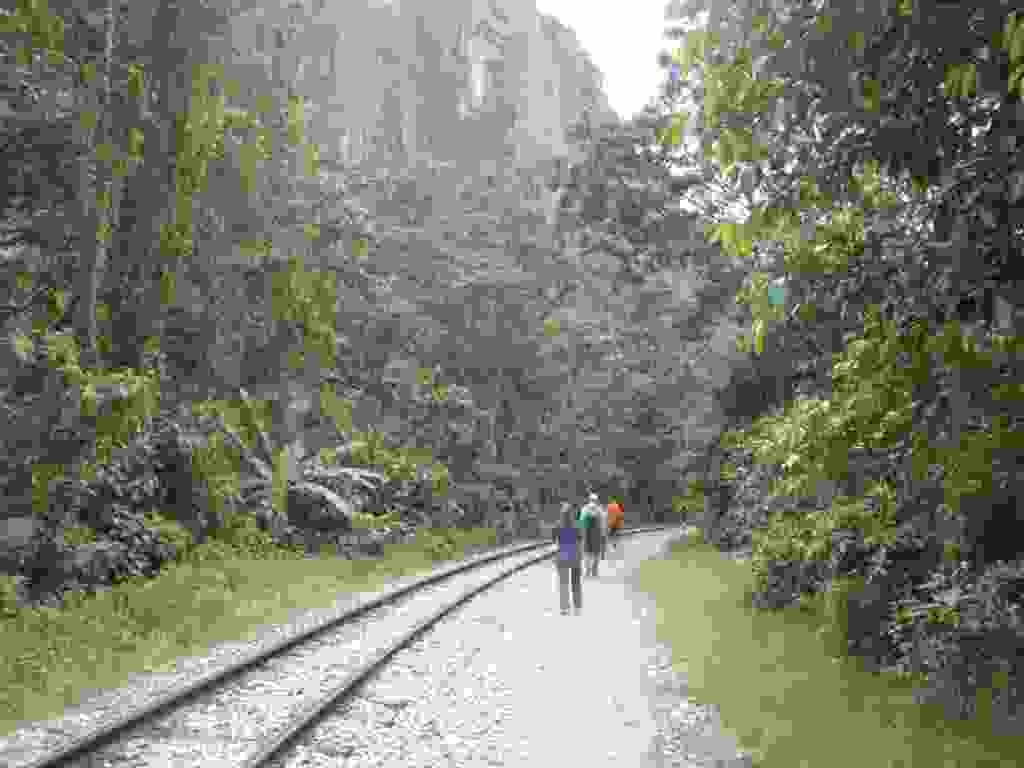
\includegraphics[width=\mywidth]{../wp-content/uploads/2015/05/P5264442-1024x768.jpg} } 
 \newline
 \newline
\centerline{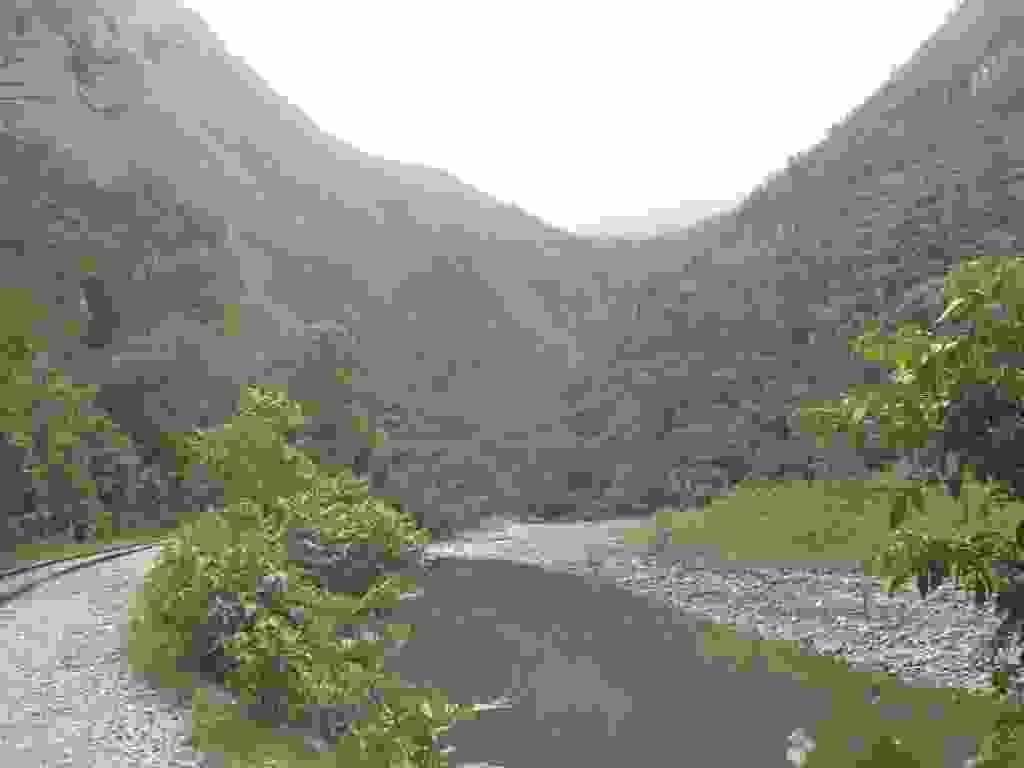
\includegraphics[width=\mywidth]{../wp-content/uploads/2015/05/P5264444-1024x768.jpg} } 
 \newline
 Ce village n'est accessible qu'en train ou à pied, on y trouve quasiment que des hôtels et des restaurants où les prix sont multipliés par 3 ou 4 par rapport au reste du Pérou. \newline
 \newline
\centerline{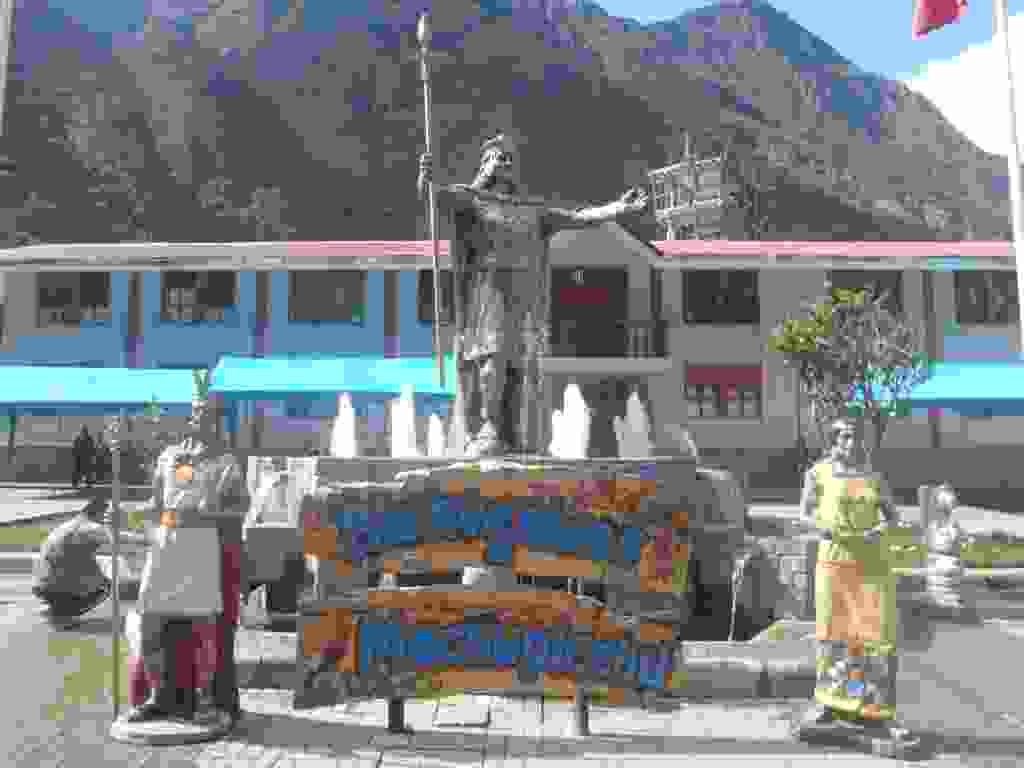
\includegraphics[width=\mywidth]{../wp-content/uploads/2015/06/P5284557-1024x768.jpg} } 
 \newline
 \newline
\centerline{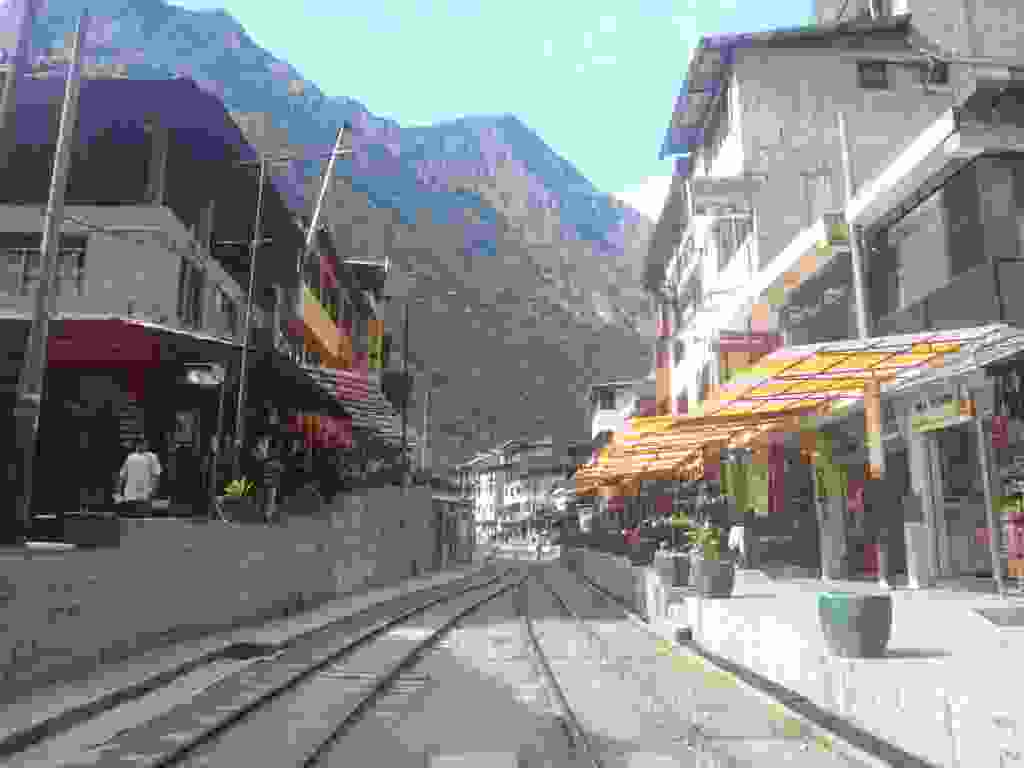
\includegraphics[width=\mywidth]{../wp-content/uploads/2015/06/P5284560-1024x768.jpg} } 
 \newline
 Jour 5 : \newline
 Départ à 4h30 pour arriver au premier point de contrôle du Machu Picchu avant l'ouverture à 5h. \newline
 1h de montée à la frontale jusqu'à l'entrée du Machu Picchu qui ouvre à 6h. \newline
 Premieres photos du Machu Picchu encore presque désert à cette heure là. \newline
 \newline
\centerline{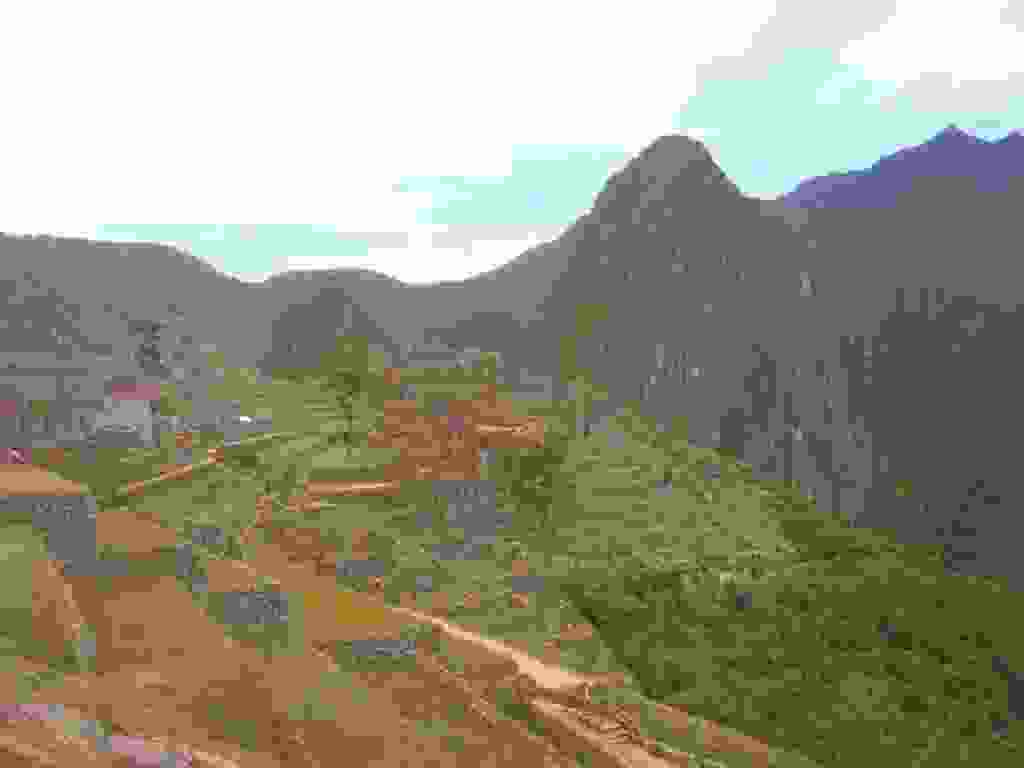
\includegraphics[width=\mywidth]{../wp-content/uploads/2015/06/P5274452-1024x768.jpg} } 
 \newline
 \newline
\centerline{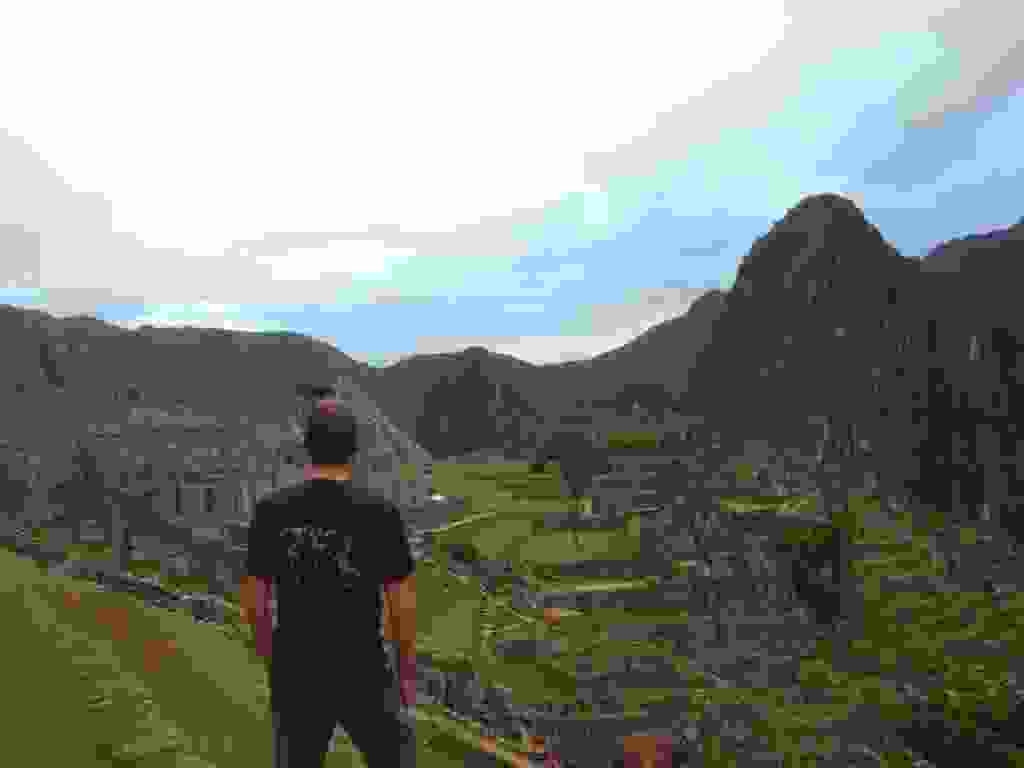
\includegraphics[width=\mywidth]{../wp-content/uploads/2015/06/P5274457-1024x768.jpg} } 
 \newline
 Le lever du soleil sur les montagnes. \newline
 \newline
\centerline{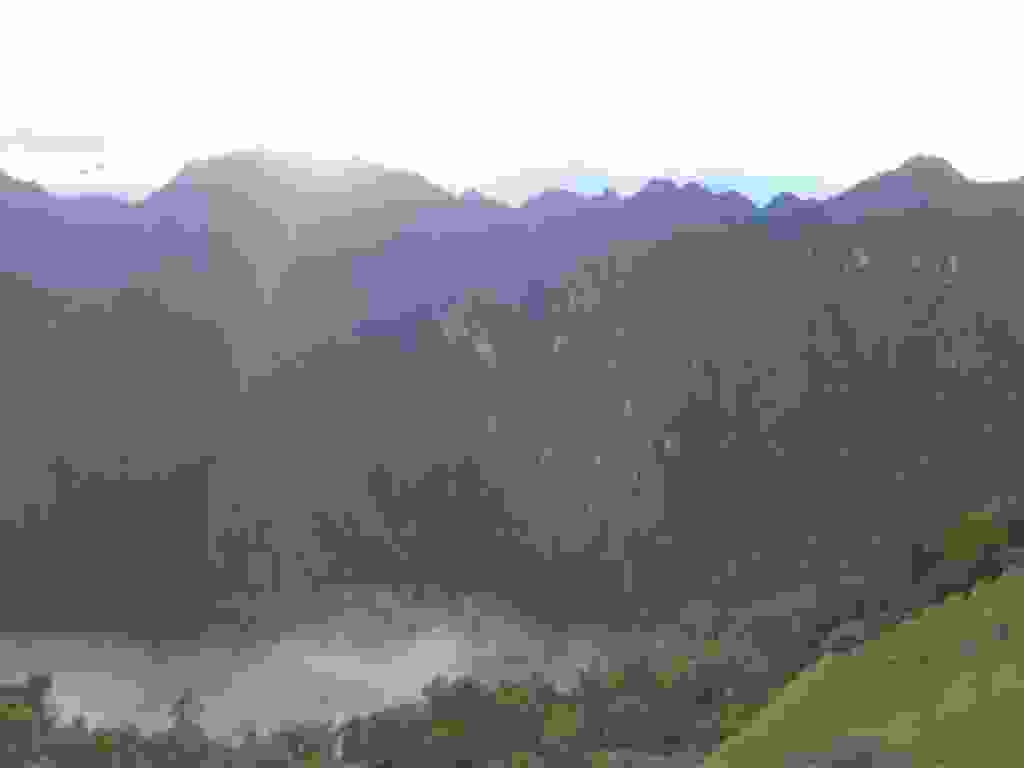
\includegraphics[width=\mywidth]{../wp-content/uploads/2015/06/P5274465-1024x768.jpg} } 
 \newline
 Petite visite guidée pour voir quelques endroits intéressants : \newline
 \newline
\centerline{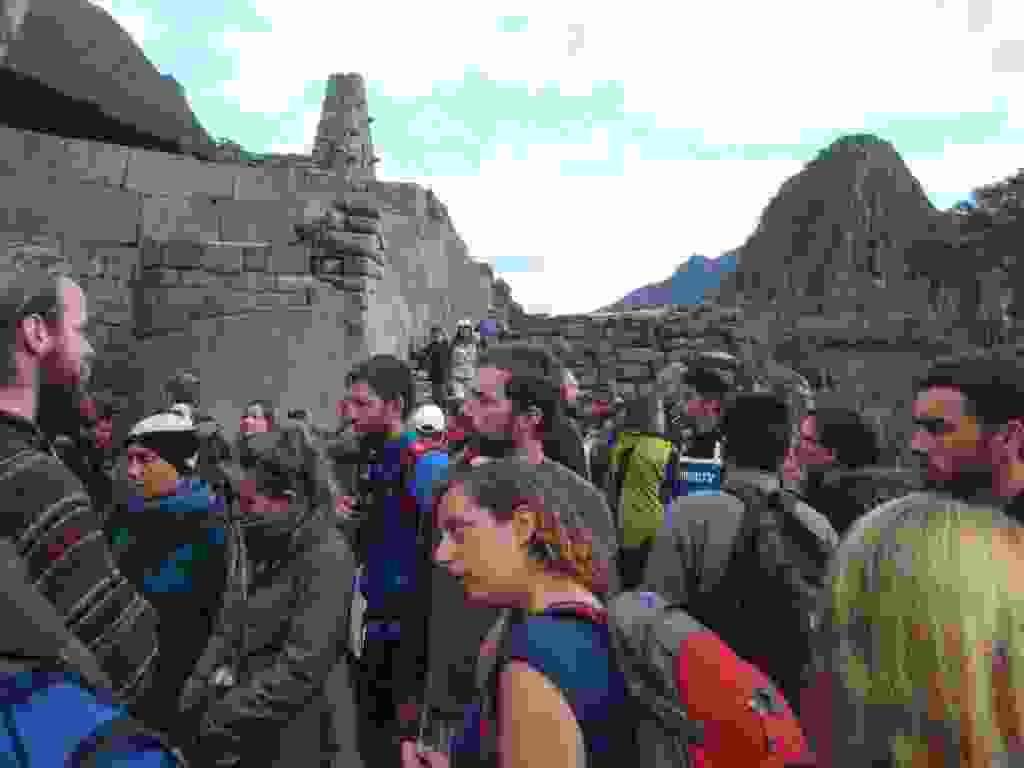
\includegraphics[width=\mywidth]{../wp-content/uploads/2015/06/P5274466-1024x768.jpg} } 
 \newline
 Le temple du soleil. \newline
 \newline
\centerline{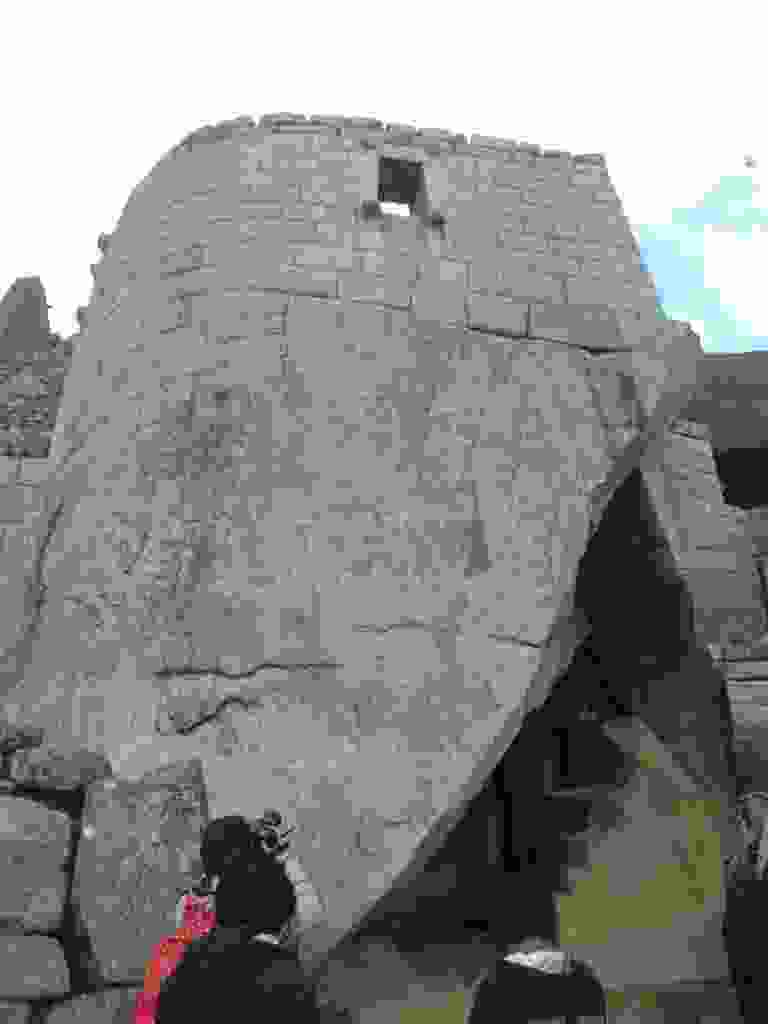
\includegraphics[width=\mywidth]{../wp-content/uploads/2015/06/P5274464-768x1024.jpg} } 
 \newline
 \newline
\centerline{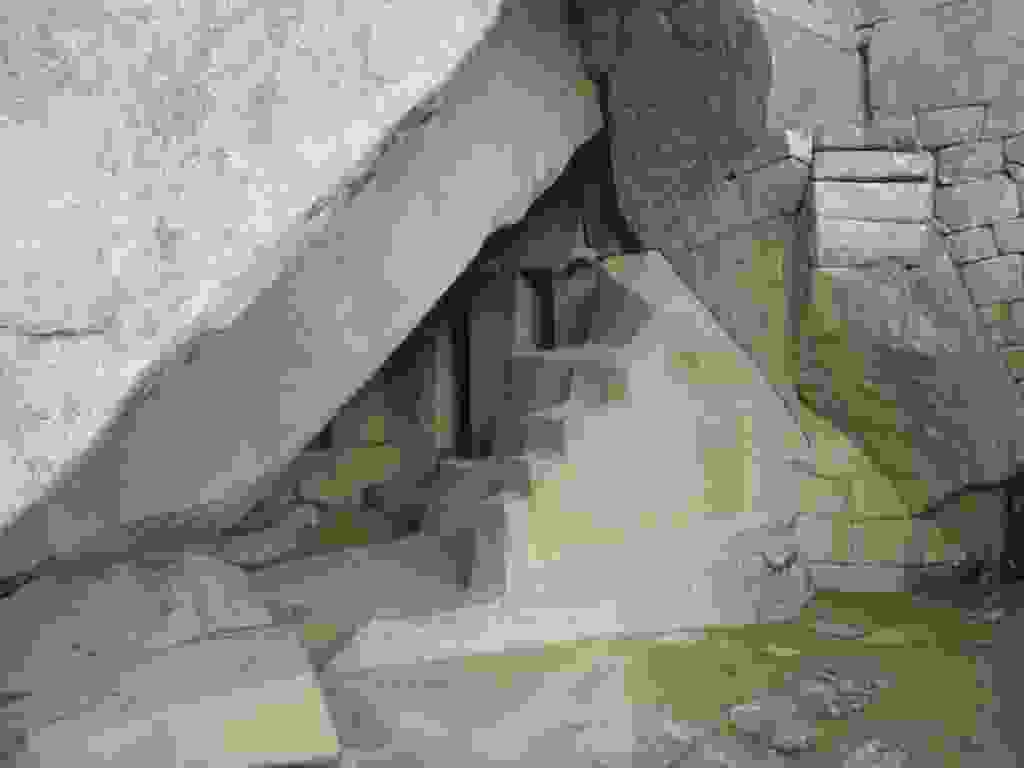
\includegraphics[width=\mywidth]{../wp-content/uploads/2015/06/P5274462-1024x768.jpg} } 
 \newline
 Les miroirs d'eau. \newline
 \newline
\centerline{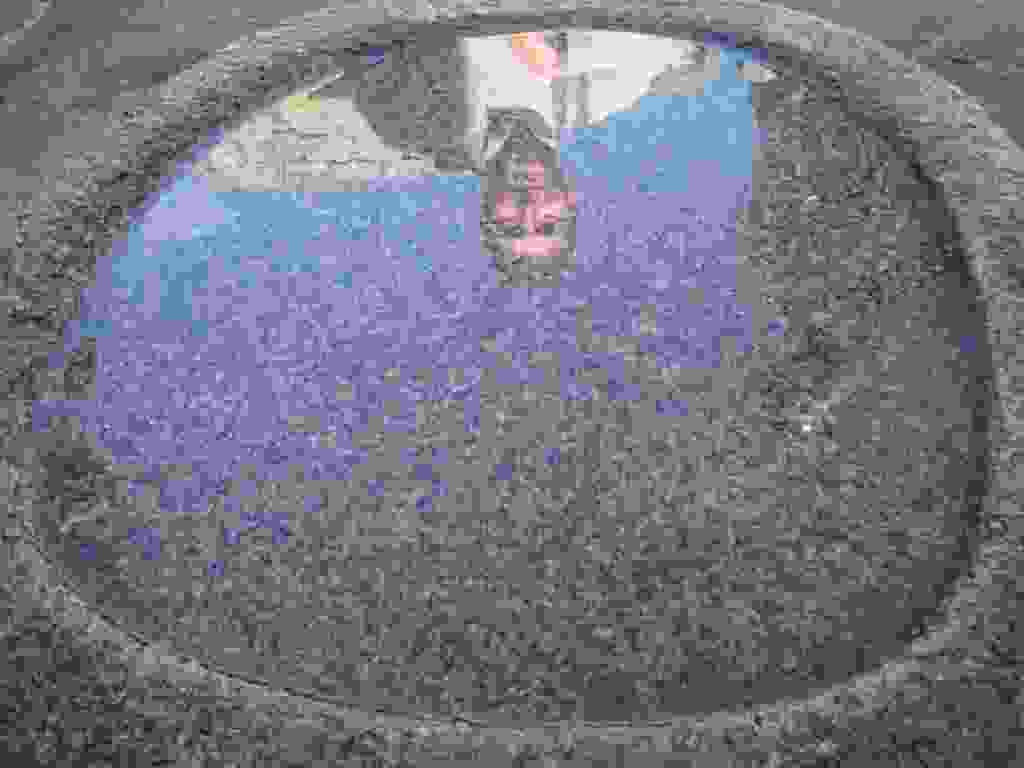
\includegraphics[width=\mywidth]{../wp-content/uploads/2015/06/P5274487-1024x768.jpg} } 
 \newline
 Temple des 3 fenetres. \newline
 \newline
\centerline{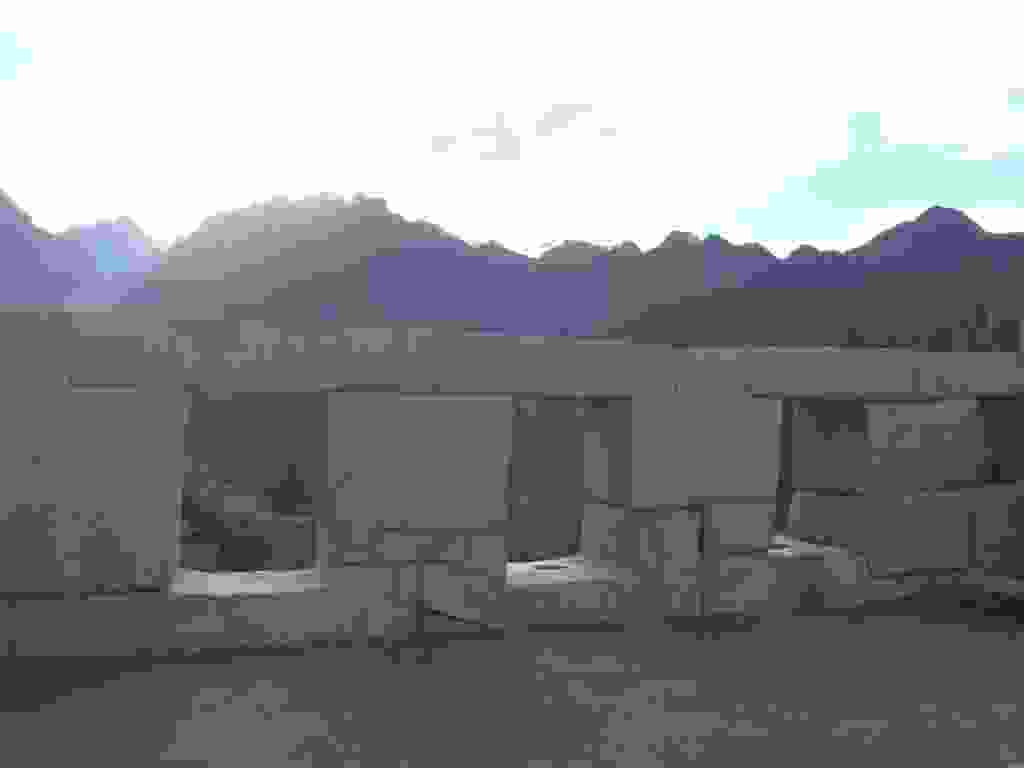
\includegraphics[width=\mywidth]{../wp-content/uploads/2015/06/P5274480-1024x768.jpg} } 
 \newline
 Temple principal. \newline
 \newline
\centerline{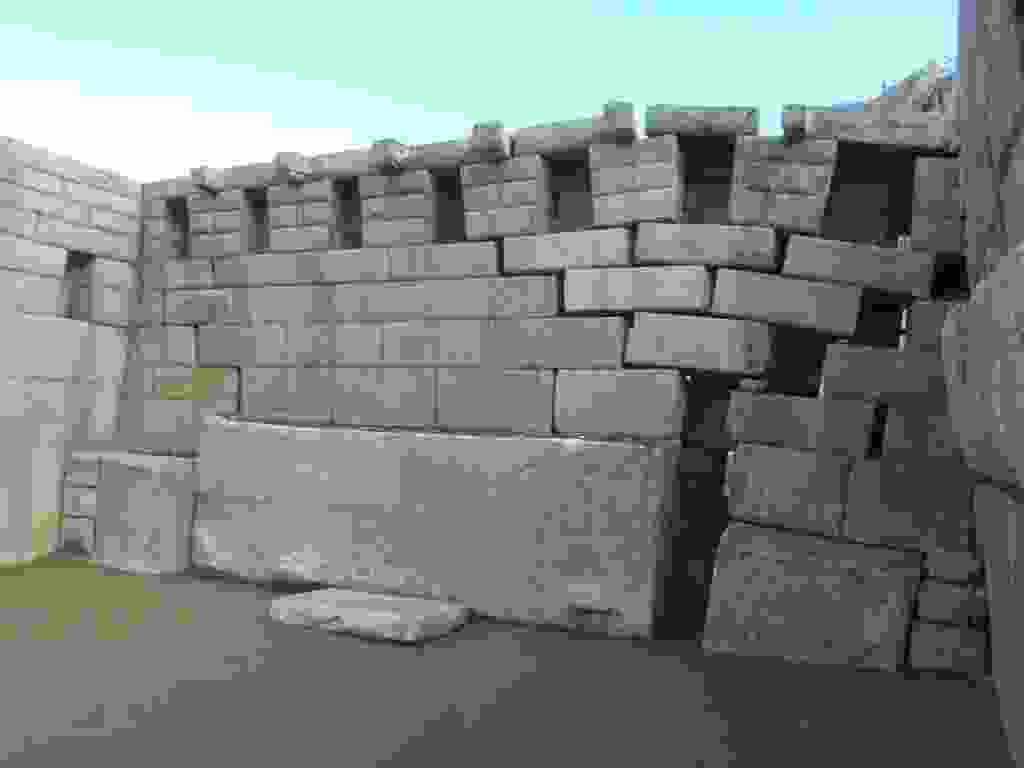
\includegraphics[width=\mywidth]{../wp-content/uploads/2015/06/P5274478-1024x768.jpg} } 
 \newline
 Des murs incas antisismiques : du bon boulot. \newline
 \newline
\centerline{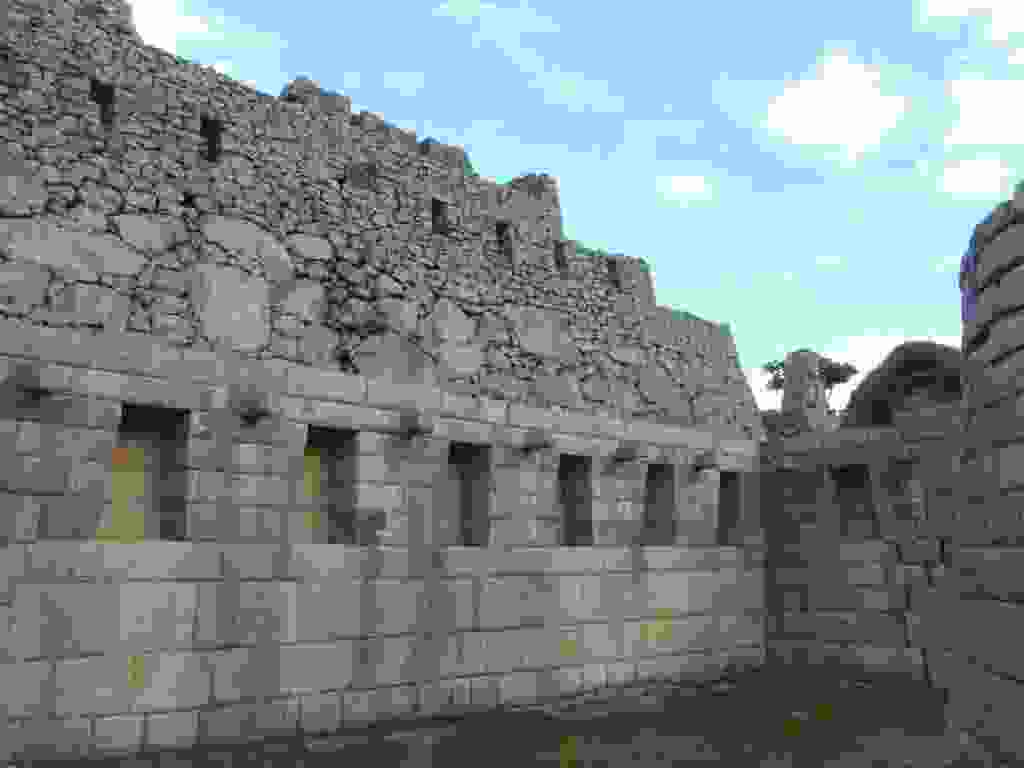
\includegraphics[width=\mywidth]{../wp-content/uploads/2015/06/P5274468-1024x768.jpg} } 
 \newline
 \newline
\centerline{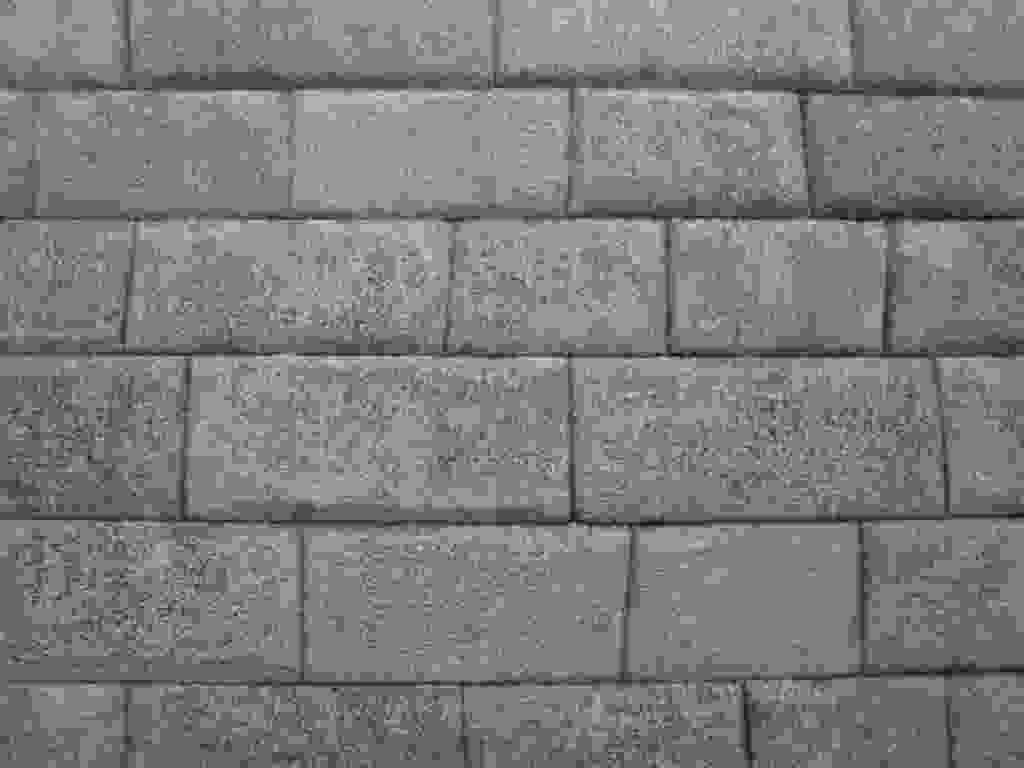
\includegraphics[width=\mywidth]{../wp-content/uploads/2015/06/P5274469-1024x768.jpg} } 
 \newline
 Un petit tour du site : \newline
 \newline
\centerline{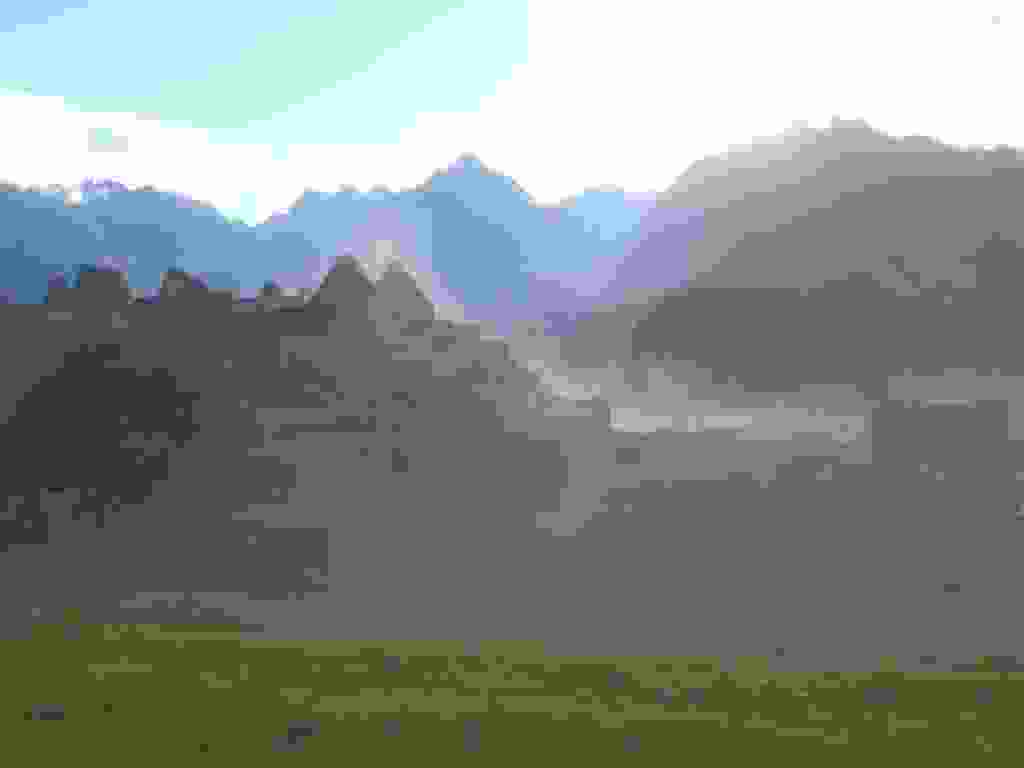
\includegraphics[width=\mywidth]{../wp-content/uploads/2015/06/P5274483-1024x768.jpg} } 
 \newline
 \newline
\centerline{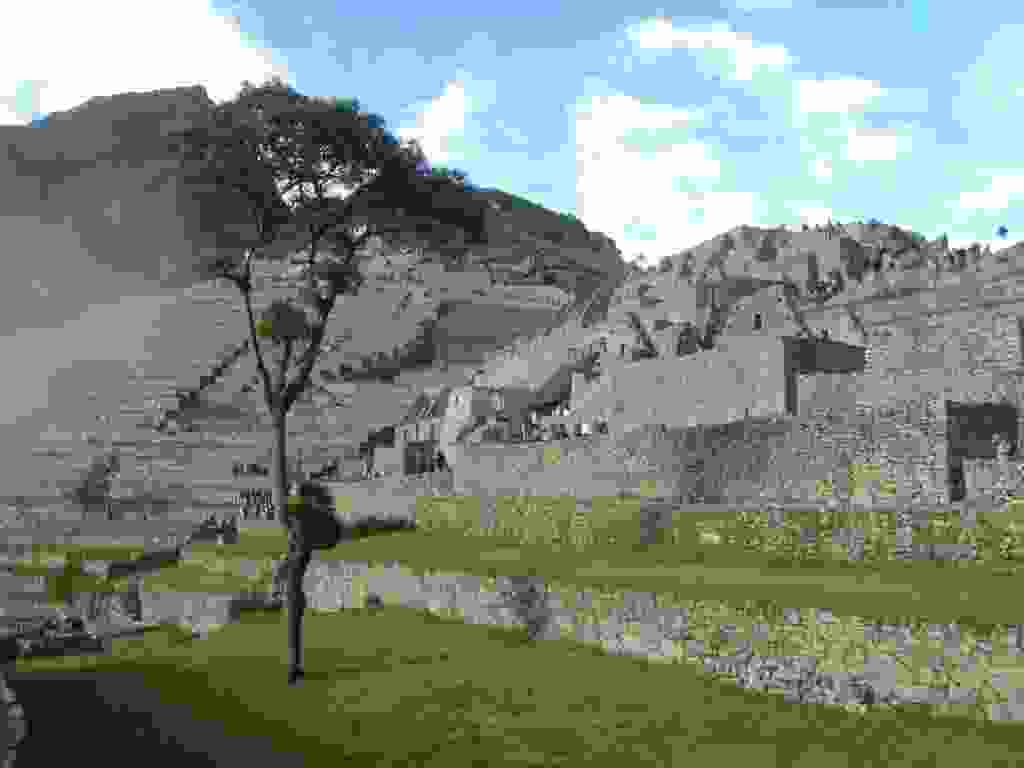
\includegraphics[width=\mywidth]{../wp-content/uploads/2015/06/P5274484-1024x768.jpg} } 
 \newline
 \newline
\centerline{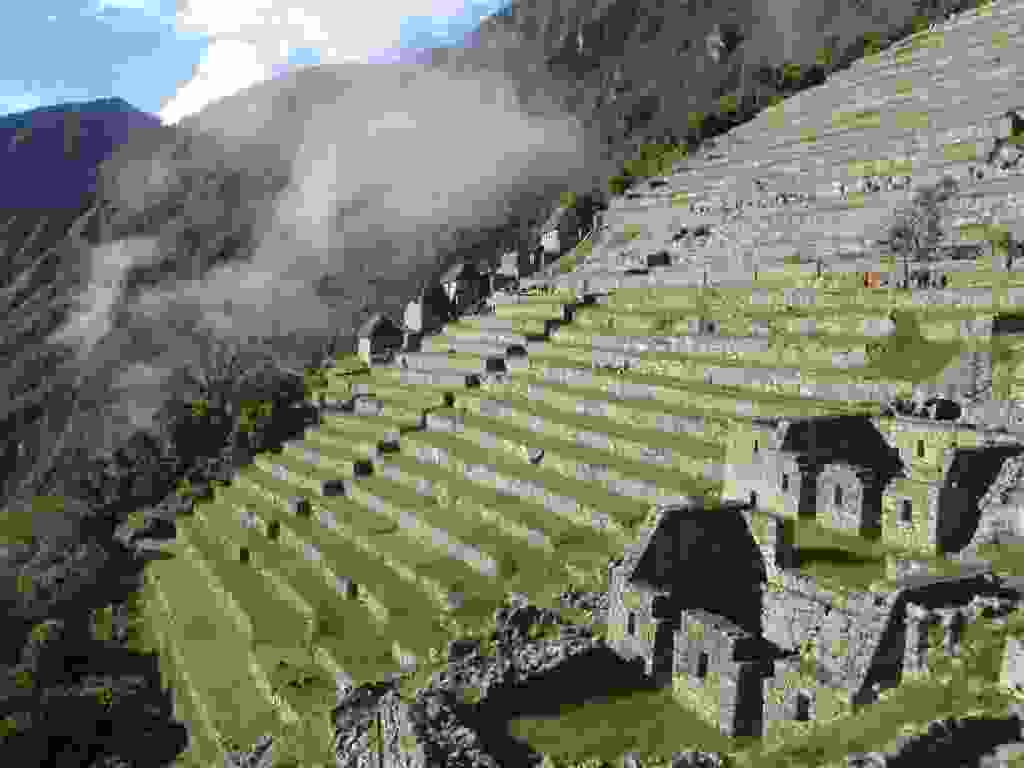
\includegraphics[width=\mywidth]{../wp-content/uploads/2015/06/P5274490-1024x768.jpg} } 
 \newline
 \newline
\centerline{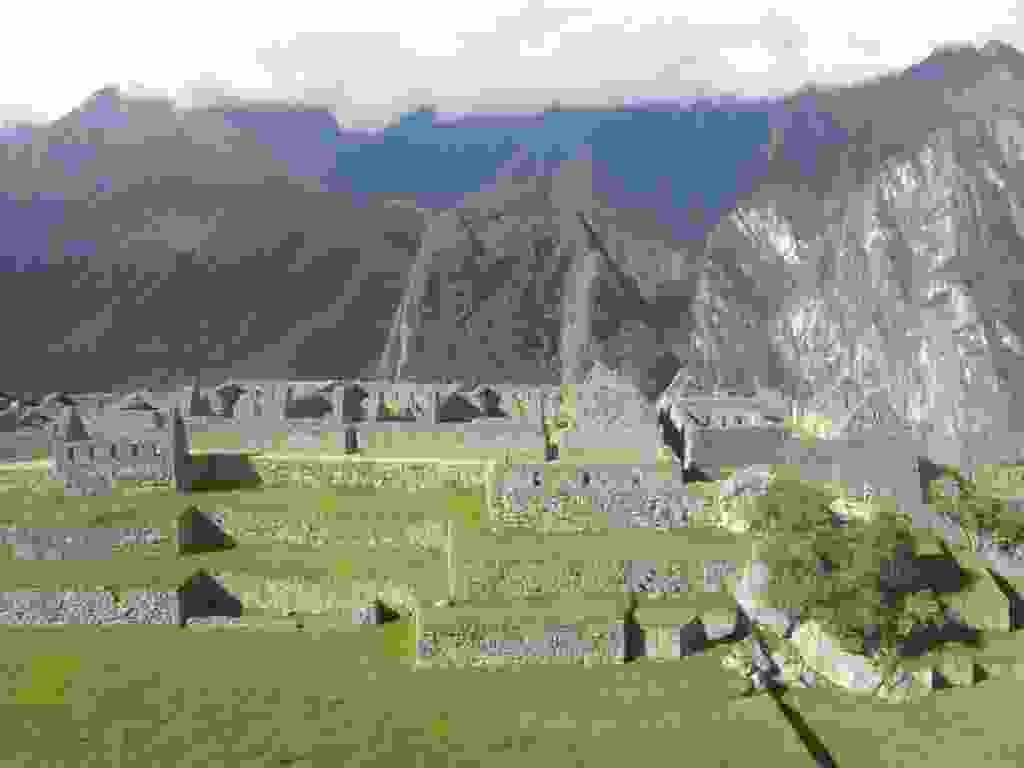
\includegraphics[width=\mywidth]{../wp-content/uploads/2015/06/P5274548-1024x768.jpg} } 
 \newline
 \newline
\centerline{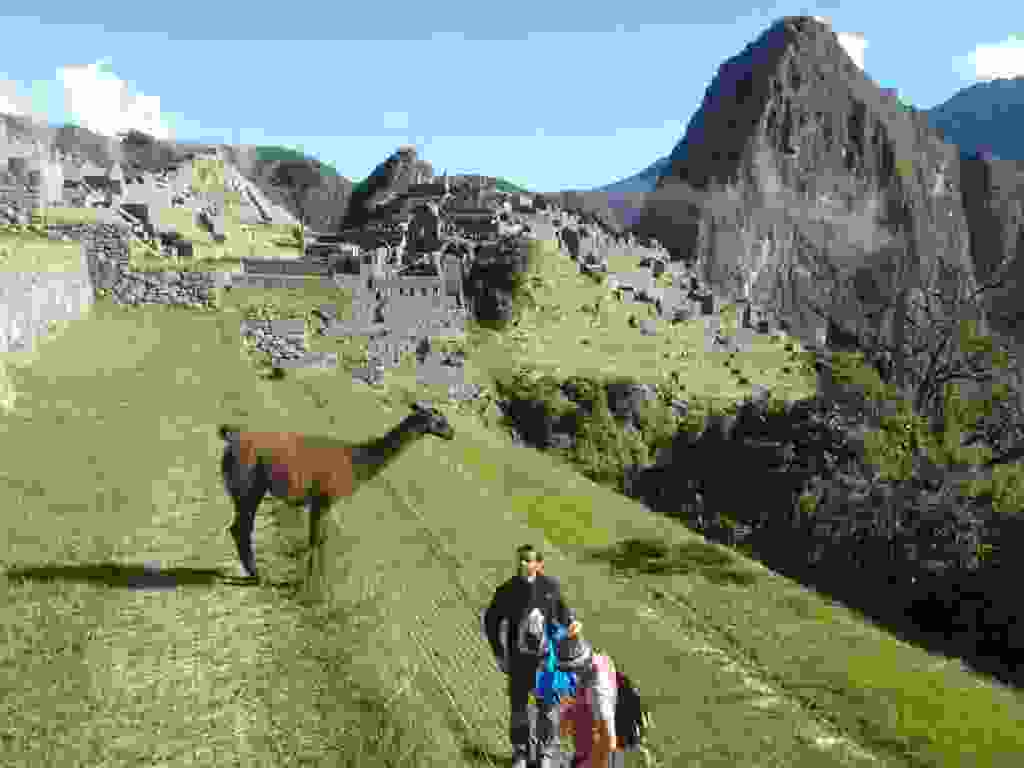
\includegraphics[width=\mywidth]{../wp-content/uploads/2015/06/P5274496-1024x768.jpg} } 
 \newline
 La photo avant de dire au revoir a notre guide. \newline
 \newline
\centerline{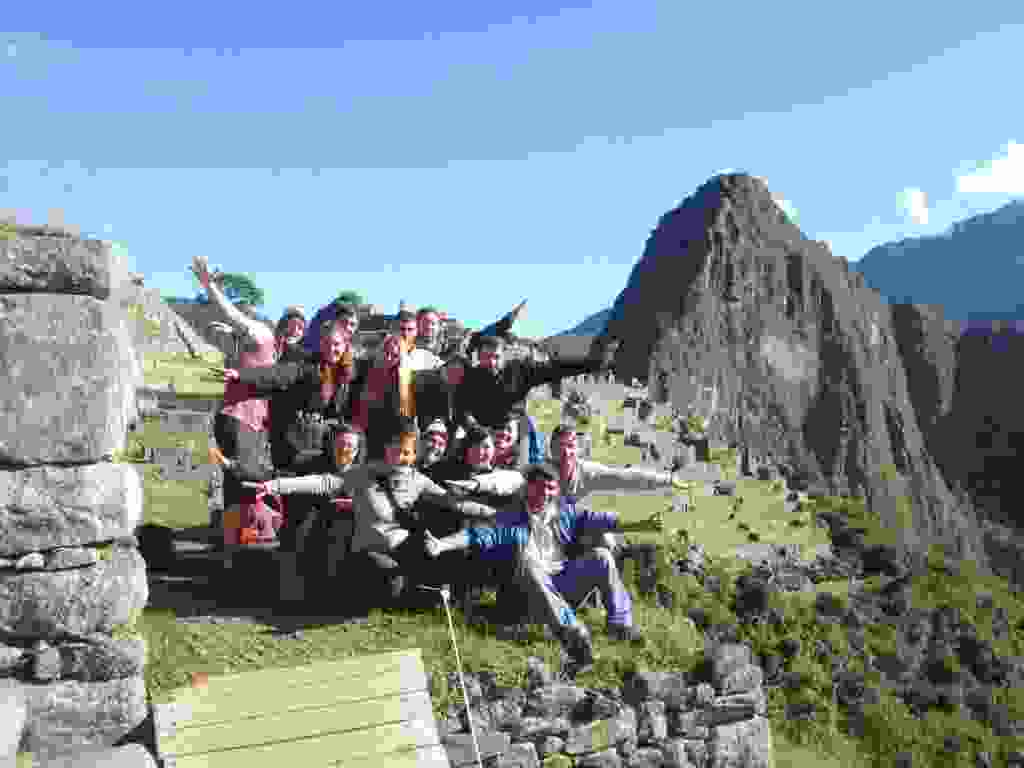
\includegraphics[width=\mywidth]{../wp-content/uploads/2015/06/P5274493-1024x768.jpg} } 
 \newline
 On monte ensuite en haut de la montagne du Machu Picchu : 1h30 de marches en pierre. \newline
 \newline
\centerline{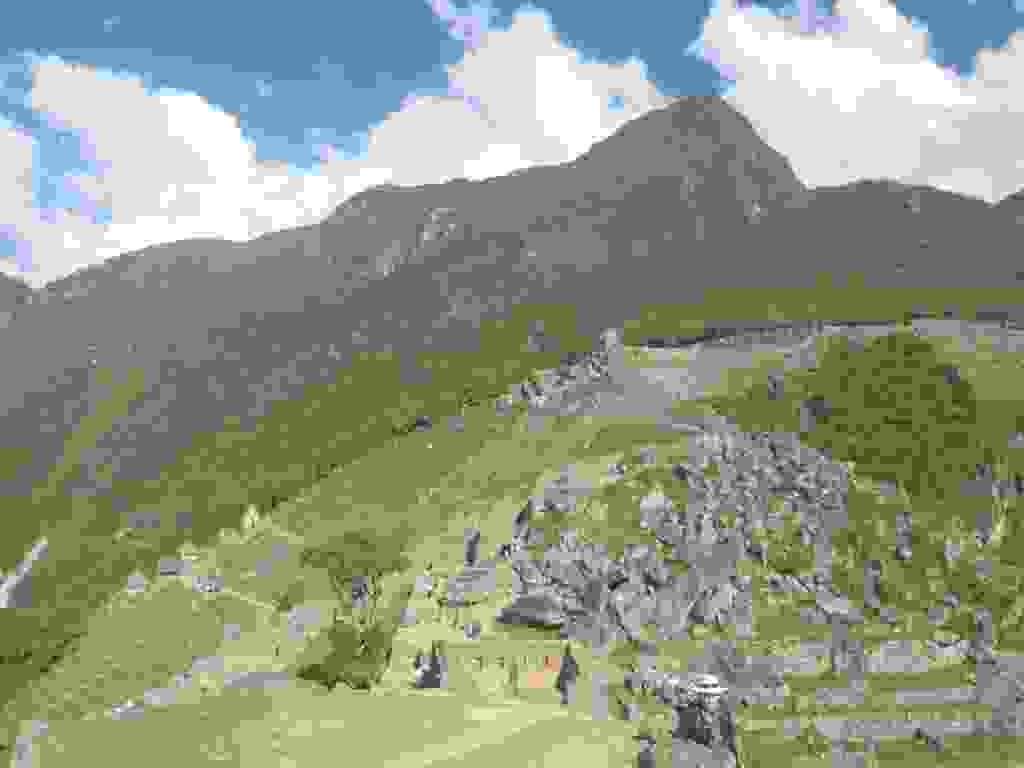
\includegraphics[width=\mywidth]{../wp-content/uploads/2015/06/P5274549-1024x768.jpg} } 
 \newline
 \newline
\centerline{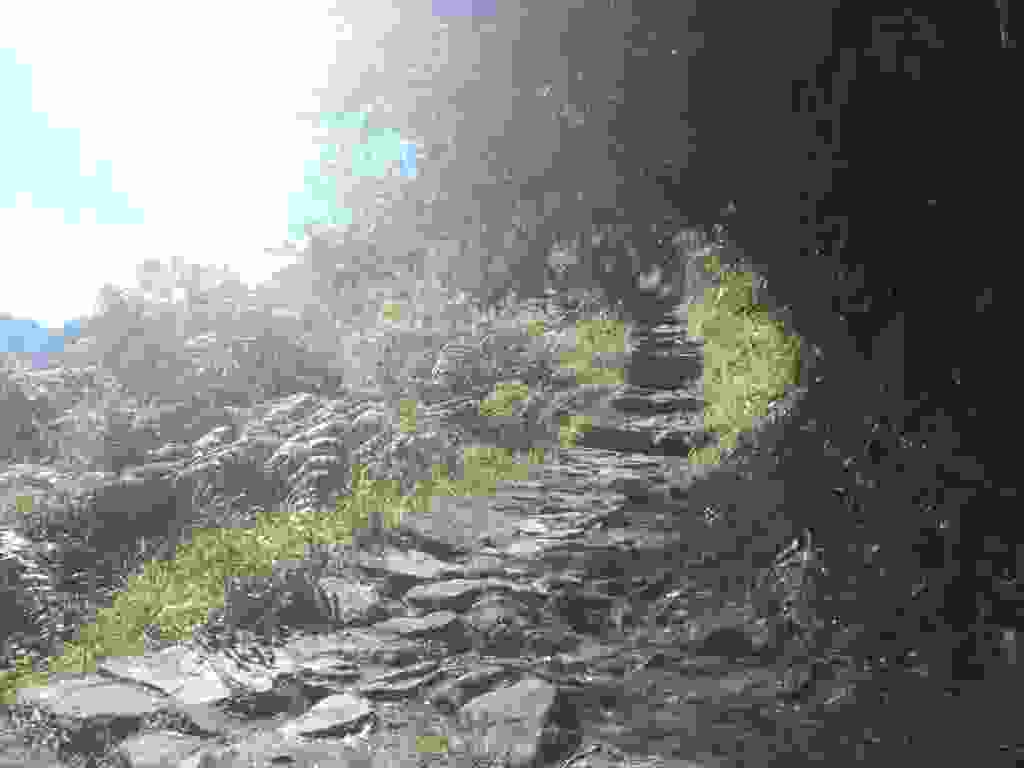
\includegraphics[width=\mywidth]{../wp-content/uploads/2015/06/P5274507-1024x768.jpg} } 
 \newline
 D´en haut, la vue est grandiose. \newline
 \newline
\centerline{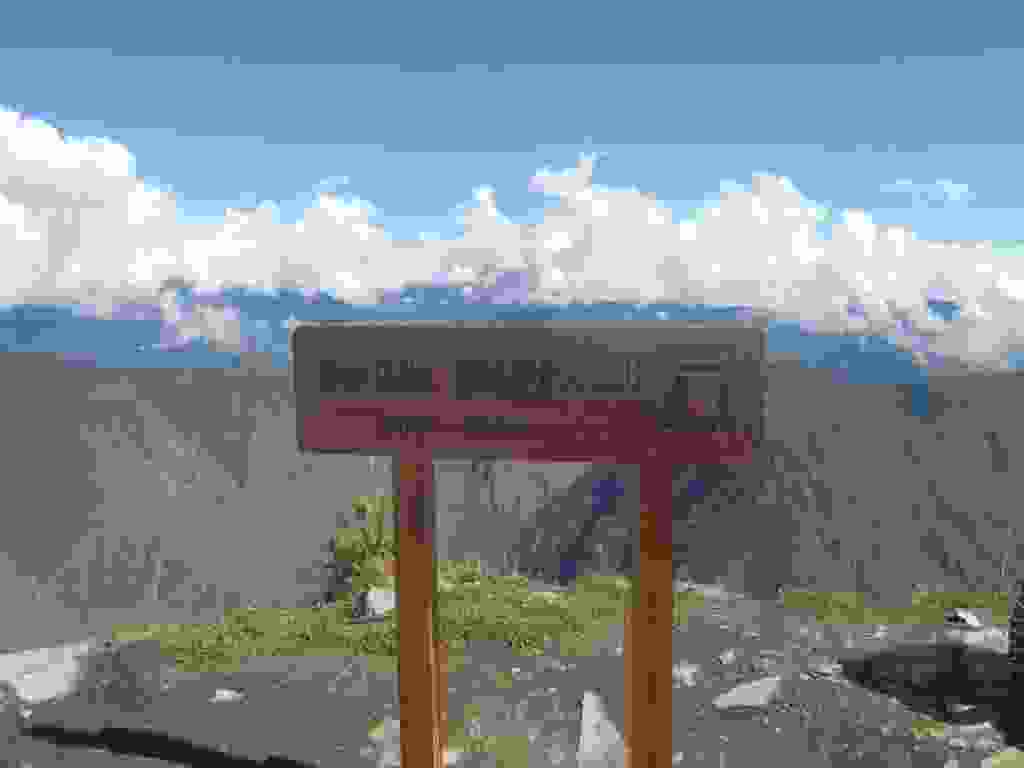
\includegraphics[width=\mywidth]{../wp-content/uploads/2015/06/P5274513-1024x768.jpg} } 
 \newline
 \newline
\centerline{\includegraphics[width=\mywidth]{../wp-content/uploads/2015/06/P5274511-1024x768.jpg} } 
 \newline
 \newline
\centerline{\includegraphics[width=\mywidth]{../wp-content/uploads/2015/06/P5274508-1024x768.jpg} } 
 \newline
 \newline
\centerline{\includegraphics[width=\mywidth]{../wp-content/uploads/2015/06/P5274509-1024x768.jpg} } 
 \newline
 \newline
\centerline{\includegraphics[width=\mywidth]{../wp-content/uploads/2015/06/P5274521-768x1024.jpg} } 
 \newline
 \newline
\centerline{\includegraphics[width=\mywidth]{../wp-content/uploads/2015/06/P5274515-1024x768.jpg} } 
 \newline
 Le pont incas à 20 min de marche. \newline
 \newline
\centerline{\includegraphics[width=\mywidth]{../wp-content/uploads/2015/06/P5274537-1024x768.jpg} } 
 \newline
 Jour 6 : \newline
 Retour à Hidroelectrica par la voie ferrée puis 7h de bus pour rentrer à Cusco. \newline

\newpage
 
